\chapter{Aplicaciones entre Espacios Topológicos}

\section{Continuidad}

Para $\bb{R}$, decíamos que $f:\bb{R}\to \bb{R}$ es continua en $x_0\in \bb{R}$ si:
\begin{equation*}
    \forall \veps\in \bb{R}^+,~\exists \delta\in \bb{R}^+ \mid \forall x \text{ con } |x-x_0|<\delta \text{ se tiene que } |f(x)-f(x_0)|<\veps
\end{equation*}

Para espacios métricos, decíamos que dada $f:(X,d)\to (Y,d')$ es continua en $x_0\in X$ si:
\begin{equation*}
    \forall \veps\in \bb{R}^+,~\exists \delta\in \bb{R}^+ \mid f[B(x_0,\delta)]\subset B[f(x_0),\veps]
\end{equation*}

Esto es equivalente a decir que:
\begin{equation*}
    \forall N\in N_{f(x_0)} \text{ se tiene que } f^{-1}(N)\in N_{x_0}
\end{equation*}


Esta definición se generaliza para cualquier espacio topológico:
\begin{definicion}[Continuidad]
    Sea $f:(X,\T)\to (Y,\T')$ una aplicación entre dos espacios topológicos, y sea $x_0\in X$. Decimos que $f$ es continua en $x_0$ si para todo $N'\in N_{f(x_0)}$ entorno de $f(x_0)$ existe un entorno $N\in N_{x_0}$ entorno de $x_0$ tal que $f(N)\subset N'$. Es decir,
    \begin{equation*}
        \forall N'\in N_{f(x_0)},~~\exists N\in N_{x_0} \text{ con } f(N)\subset N'
    \end{equation*}
\end{definicion}

\begin{observacion}
    Recordamos las siguientes nociones de Álgebra I. Sea $f:X\to Y$. Entonces, dado $W\subset X$, $Z\subset Y$, se tiene que:
    \begin{enumerate}
        \item $W\subset f^{-1}(f(W))$. Además, si es inyectiva se da la igualdad.

        \item $f(f^{-1}(Z))\subset Z$. Además, si es sobreyectiva se da la igualdad.
    \end{enumerate}
\end{observacion}


Vamos a caracterizar la definición de continuidad en términos de bases, bases de entornos y también en términos de la preimagen de $f$:
\begin{prop}[Caracterización de la continuidad]\label{prop:Caract_ContinuidadPto}
    Sea $f:(X,\T)\to (Y,\T')$ una aplicación entre dos espacios topológicos, y sea $x_0\in X$. Entonces, son equivalentes:
    \begin{enumerate}
        \item $f$ es continua en $x_0$.
        \item Dadas $\beta_{x_0}$ base de entornos de $x_0$ y $\beta_{f(x_0)}$ base de entornos de $f(x_0)$, para cualquier $V'\in \beta_{f(x_0)}$ existe $V\in \beta_{x_0}$ tal que $f(V)\subset V'$. Es decir,
        \begin{equation*}
            \forall V'\in \beta_{f(x_0)},~~\exists V\in \beta_{x_0} \mid f(V)\subset V'
        \end{equation*}
        \item La preimagen de cualquier entorno de $f(x_0)$ es un entorno de $x_0$. Es decir,
        \begin{equation*}
            \forall N\in N_{f(x_0)}\text{ se tiene que } f^{-1}(N)\in N_{x_0}
        \end{equation*}
    \end{enumerate}
\end{prop}
\begin{proof}\
    \begin{description}
        \item[$1\Longrightarrow 2)$] Dado $V'\in \beta_{f(x_0)}$, en particular $V'\in N_{f(x_0)}$. Como $f$ es continua en $x_0$ se tiene que $\exists N\in N_{x_0}$ tal que $f(N)\subset V'$. 
        
        Por ser $\beta_{x_0}$ una base de entornos, por definición $\exists V\in \beta_{x_0}$ tal que $V\subset N$. Por tanto, se tiene que $f(V)\subset f(N)\subset V'$, demostrando así 2).
    
        \item[$2\Longrightarrow 3)$] Consideramos las bases de entornos triviales dadas por todos los entornos. Entonces, dado $N\in N_{f(x_0)}=\beta_{f(x_0)}$, por 2) se tiene que $\exists V\in N_{x_0}=\beta_{x_0}$ tal que $f(V)\subset N$.
        
        Entonces, $V\subset f^{-1}(f(V))\subset f^{-1}(N)$. Como $V\in N_{x_0}$, y $V\subset f^{-1}(N)$, tenemos que $f^{-1}(N)\in N_{x_0}$.

        \item[$3\Longrightarrow 1)$] Dado $N'\in N_{f(x_0)}$, por 3) tenemos que $f^{-1}(N')\in N_{x_0}$. Consideramos $N=~f^{-1}(N')$. Entonces $f(N)=f(f^{-1}(N'))\subset N'$, por lo que tenemos que $f$ es continua en $x_0$.
    \end{description}
\end{proof}

\begin{definicion}[Continuidad global] Sea $f:(X,\T)\to (Y,\T')$ una aplicación entre espacios topológicos. Decimos que $f$ es continua si $f$ es continua en todo $x\in X$.
\end{definicion}

\begin{prop}[Caracterización de la continuidad global]\label{prop:Caract_ContinuidadGlobal}
    Sea una aplicación entre dos espacios topológicos $f:(X,\T)\to (Y,\T')$. Entonces, son equivalentes:
    \begin{enumerate}
        \item $f$ es continua.
        \item La preimagen de todo abierto de $\T'$ es un abierto de $\T$. Es decir,
        \begin{equation*}
            f^{-1}(U')\in \T, \qquad \forall U'\in \T'
        \end{equation*}
        \item La preimagen de todo abierto básico (de una base dada) es abierto. Es decir, dada $\cc{B}'$ base de $\T'$, se cumple que:
        \begin{equation*}
            f^{-1}(B')\in \T, \qquad \forall B'\in \cc{B}'
        \end{equation*}

        \item La preimagen de todo elemento de una subbase fijada de $\T'$ es un abierto. Es decir, dada $S$ subbase de $\T'$, se tiene que:
        \begin{equation*}
            f^{-1}(A)\in \T, \qquad \forall A\in S
        \end{equation*}

        \item La preimagen de todo cerrado de $\T'$ es un cerrado de $\T$. Es decir,
        \begin{equation*}
            f^{-1}(C)\in C_\T, \qquad \forall C'\in C_{\T'}
        \end{equation*}

        \item Dado $D\subset X$, la imagen de su adherencia ha de estar contenida en la adherencia de su imagen. Es decir,
        \begin{equation*}
            f\left(\ol{D}\right)\subset \ol{f(D)},\qquad \forall D\subset X
        \end{equation*}
    \end{enumerate}
\end{prop}
\begin{proof}\
    \begin{description}
        \item[$1\Longrightarrow 2)$] Dado $U\in \T'$, por la Proposición \ref{prop:CaractAbiertos_conEntornos}, tenemos que $U\in N_x~\forall x\in U$. En particular, dado $x_0\in f^{-1}(U)\subset X$, como $U\in N_{f(x_0)}$ y $f$ es continua en $x_0$, tenemos que $f^{-1}(U)\in N_{x_0}$.

        Por tanto, tenemos que $f^{-1}(U)\in N_{x_0}~\forall x_0\in f^{-1}(U)$. Por tanto, por la proposición \ref{prop:CaractAbiertos_conEntornos}, tenemos que $f^{-1}(U)\in \T$, quedando demostrada esta implicación.

        \item[$2\Longrightarrow 1)$] Tenemos que probar que $f$ es continua; es decir, si $x_0\in X$, entonces $f$ es continua en $x_0$.

        Dado $x_0\in X$, por la Proposición \ref{prop:Caract_ContinuidadPto}, tenemos que demostrar que si $N\in N_{f(x_0)}$, entonces $f^{-1}(N)\in N_{x_0}$.

        Como $N\in N_{f(x_0)}$, $\exists U\in \T'$ tal que $f(x_0)\in U\subset N$. Veamos ahora que $f^{-1}(N)\in N_{x_0}$:
        \begin{equation*}
            x_0\in f^{-1}(f(x_0))\subset f^{-1}(U)\subset f^{-1}(N) \in N_{x_0}
        \end{equation*}
        donde sabemos que es un entorno ya que, usando 2), tenemos que $f^{-1}(U)\in \T$. 


        \item[$2\Longrightarrow 3)$] TERMINAR
        \item[$3\Longrightarrow 4)$]
        \item[$4\Longrightarrow 1)$]

        \item[$2\Longrightarrow 5)$]
        \item[$5\Longrightarrow 2)$]

        \item[$5\Longrightarrow 6)$] Sea $D\subset X$. Entonces, $\ol{f(D)}\in C_{\T'}$. Por 5), se tiene que $f^{-1}\left(\ol{f(D)}\right)\in C_\T$.

        Como $f(D)\subset \ol{f(D)}$, se tiene que $D\subset f^{-1}(f(D))\subset f^{-1}\left(\ol{f(D)}\right)\in C_\T$; y como la adherencia es el menor cerrado que contiene al conjunto, $\ol{D}\subset f^{-1}\left(\ol{f(D)}\right)$, por lo que $f\left(\ol{D}\right)\subset f\left[f^{-1}\left(\ol{f(D)}\right)\right]\subset \ol{f(D)}$, demostrando así lo pedido.
        
        \item[$6\Longrightarrow 5)$] Sea $C\in C_{\T'}$. Usando 6) para $D=f^{-1}(C)$, tenemos que: $$f\left(\ol{f^{-1}(C)}\right)\subset \ol{f(f^{-1}(C))}\subset \ol{C}\AstIg C$$
        donde en $(\ast)$ hemos usado que $C\in C_{\T'}$. Además, $\ol{f^{-1}(C)}\subset f^{-1}\left[f\left(\ol{f^{-1}(C)}\right)\right]$, por lo que:
        \begin{equation*}
            \ol{f^{-1}(C)}\subset f^{-1}\left[f\left(\ol{f^{-1}(C)}\right)\right] \subset f^{-1}(C)
        \end{equation*}
        

        Por tanto, $f^{-1}(C)=\ol{f^{-1}(C)}$, por lo que $f^{-1}(C)\in C_\T$.
        
    \end{description}
\end{proof}


\begin{observacion}
    Si $f:(X,\T)\to (\bb{R},\T_u)$ es una aplicación continua. Entonces, por la proposición anterior se tiene que:
    \begin{gather*}
        f^{-1}(a)=\{x\in X\mid f(x)=a\}\in C_\T\\
        f^{-1}(]a,b[)=\{x\in X\mid a<f(x)<b\}\in \T.
    \end{gather*}
\end{observacion}

\begin{ejemplo} Algunos ejemplos de aplicaciones continuas entre espacios topológicos son:
    \begin{enumerate}
        \item Hay que observar que las aplicaciones continuas entre espacios métricos son aplicaciones continuas entre los espacios topológicos correspondientes a esas distancias.

        \item Cualquier aplicación $f$ cuyo dominio sea $(X,\T_{disc})$ o cuyo codominio sea $(Y,\T_t)$, siempre será continua.

        Para el primer caso, tenemos que $f^{-1}(U)\in \T_{disc}=\cc{P}(X)$ independientemente de $U\in \T'$, por lo que $f$ es continua.

        En el segundo caso, tenemos que $f^{-1}(\emptyset)=\emptyset \in \T$ y $f^{-1}(Y)=X \in \T$ independientemente de $\T$, por lo que $f$ es continua.

        \item Si $(X,\T)$ es un espacio topológico y $A\subset X$, entonces la aplicación inclusión:
        \Func{i}{\left(A,\T_{\big|A}\right)}{(X,\T)}{a}{a}
        es continua.

        Esto es claro, ya que $\forall U\in \T$ se tiene que $i^{-1}(U)=U\cap A\in \T_{\big|A}$.

        \item Sea $Id:(X,\T)\to (X,\T')$. Tenemos que $Id$ es continua si y solo si $\T'\leq \T$.

        En particular, tenemos que $Id:(\bb{R},\T_S)\to (\bb{R}\to \T_u)$ es continua.

        No obstante, $Id:(\bb{R},\T_u)\to (\bb{R}\to \T_S)$ no es continua, ya que $\T_S\not\leq \T_u$.
    \end{enumerate}
\end{ejemplo}

\begin{lema}
    La composición de aplicaciones continuas entre espacios topológicos es continua. Es decir, sean $(X,\T),(Y,\T')$ y $(Z,\T'')$ tres espacios topológicos y las siguientes aplicaciones:
    \begin{figure}[H]
        \centering
        \shorthandoff{""}
        \begin{tikzcd}[row sep=large, column sep=large]
            {(X,\T)} \arrow[r, "f"] & {(Y,\T')} \arrow[r, "g"] & {(Z,\T'')}
        \end{tikzcd}
        \shorthandon{""}
    \end{figure}

    Si $f,g$ son continuas, entonces $g\circ f$ es continua.
\end{lema}
\begin{proof}
    Para probar esto, usaremos que la imagen inversa de un abierto ha de ser un abierto. Es decir, que dado $U\in \T''$, entonces $(g\circ f)^{-1}(U)\in \T$. Tenemos que:
    \begin{equation*}
        (g\circ f)^{-1}(U) = (f^{-1}\circ g^{-1})(U) = (f^{-1} (g^{-1}(U))\in \T
    \end{equation*}
    donde he aplicado que $g^{-1}(U)\in \T'$ por ser $g$ continua, por lo que su preimagen por $f$ está en $\T$ por ser $f$ continua.
\end{proof}

\begin{coro}
    La restricción en el dominio de una aplicación continua entre espacios topológicos es continua. Es decir, si $f:(X,\T)\to (Y,\T')$ es continua, dado $A\subset X$ tenemos que $f_{\big| A}:(A,\T_A)\to (Y,\T')$ es continua.
\end{coro}
\begin{proof}
    Tenemos el siguiente caso:
    \begin{figure}[H]
        \centering
        \shorthandoff{""}
        \begin{tikzcd}[row sep=large, column sep=large]
            {(A,\T_A)} \arrow[r, "i", hook] & {(X,\T)} \arrow[r, "f"] & {(Y,\T')}
        \end{tikzcd}
        \shorthandon{""}
    \end{figure}
    Como la inclusión $i$ es continua siempre y sabemos que $f$ es continua, tenemos que $f\circ i = f_{\big| A}$ es continua.
\end{proof}

Tenemos el resultado análogo para restringir el codominio.
\begin{coro}
    La restricción en el codominio de una aplicación continua entre espacios topológicos es continua. Es decir, si $f:(X,\T)\to (Y,\T')$ es continua, dado $Im(f)\subset W\subset Y$ tenemos que $f:(X,\T)\to (W,\T_W)$ es continua.
\end{coro}

\begin{lema}[de pegado] Sean $(X,\T)$, $(Y,\T')$ dos espacios topológicos. Supongamos que tenemos $\{A_i\}_{i\in I}$ una familia (no necesariamente finita) de subconjuntos tal que $\emptyset\neq A_i\subset X,\forall i\in I$ y $\{f_i:A_i\to Y\}_{i\in I}$ una familia de aplicaciones. Si se verifica:
\begin{enumerate}
    \item $X=\bigcup\limits_{i\in I}A_i$.
    \item $f_i=f_j$ en $A_i\cap A_j$ para todo $i,j\in I$.
    \item $A_i\in \T~~\forall i\in I$; o bien, en el caso de que $I$ se finito, $A_i\in C_\T ~~\forall i\in I$.
    \item $f_i:(A_i,\T_{A_i})\to (Y,\T')$ es continua $\forall i\in I$.
\end{enumerate}

Entonces, la aplicación $f:(X,\T)\to (Y,\T')$ definida como $f(x)=f_i(x)$ cuando $x\in A_i$ está bien definida y es continua.
\end{lema}
\begin{proof}

    Veamos en primer lugar que $f$ está bien definida. De 2) se deduce de forma directa; ya que dado $x\in X$, en el caso de que pertenezca a más de un subconjunto su imagen ha de ser igual por 2), y en el caso de que solo pertenezca a un conjunto, como $f_i$ es una aplicación se tiene.\\

    Veamos ahora que es continua. Para ello, supongamos que la familia $\{A_i\}_{i\in I}$ es finita y de conjuntos cerrados (para abiertos la demostración en análoga).

    Sea $C'\in C_{\T'}$. Queremos probar que $f^{-1}(C)$ es cerrado en $(X,\T)$, lo que demostraría que $f$ es continua:
    \begin{multline*}
        f^{-1}(C')=X\cap f^{-1}(C') = \left(\bigcup_{i\in I}A_i\right)\cap f^{-1}(C') = \bigcup_{i\in I}\left(A_i\cap f^{-1}(C')\right)
        =\\= \bigcup_{i\in I}\left({f_{\big| A_i}}^{-1}(C')\right)
        = \bigcup_{i\in I}\left({f_i}^{-1}(C')\right) \in C_\T
    \end{multline*}
    donde tenemos que es cerrado porque ${f_i}^{-1}(C')\in C_\T$ por ser $f_i$ continua, y la unión es un cerrado ya que la unión finita de cerrados es cerrado. (Este es el aspecto en el que la demostración difiere si $A_i$ son abiertos o cerrados).
\end{proof}


\section{Aplicaciones abiertas y cerradas. Homeomorfismos}

\begin{definicion}
    Sea $f:(X,\T)\to (Y,\T')$ una aplicación entre dos espacios topológicos. Decimos que:
    \begin{enumerate}
        \item $f$ es abierta si $f(U)\in \T',~ \forall U\in \T$.
        \item $f$ es cerrada si $f(C)\in C_{\T'},~ \forall C\in C_\T$.
    \end{enumerate}
\end{definicion}

Al igual que tenemos la caracterización de la continuidad, tenemos la caracterización de que una aplicación sea abierta:
\begin{lema}
    Sea $f:(X,\T)\to (Y,\T')$ una aplicación entre dos espacios topológicos. Entonces, equivalen:
    \begin{enumerate}
        \item $f$ es abierta.
        \item $f(B)\in \T'$ para todo $B\in \cc{B}$ base de $\T$.
        \item $f(N)\in N_{f(x)}$ para todo $x\in X, N\in N_x$.
        \item $f(A^\circ)\subset [f(A)]^\circ$ para cualquier $A\subset X$.
    \end{enumerate}
\end{lema}
\begin{proof}
    TERMINAR
\end{proof}

Por último, tenemos la caracterización de que una aplicación sea cerrada:
\begin{lema}
    Sea $f:(X,\T)\to (Y,\T')$ una aplicación entre dos espacios topológicos. Entonces, equivalen:
    \begin{enumerate}
        \item $f$ es cerrada.
        \item $\ol{f(A)}\subset f\left(\ol{A}\right)$ para cualquier $A\subset X$.
    \end{enumerate}
\end{lema}
\begin{proof}
    TERMINAR
\end{proof}


\begin{ejemplo} Veamos algunos ejemplos de aplicaciones abiertas y cerradas:
\begin{enumerate}
    \item Sea la siguiente aplicación:
    \Func{f}{\left(\bb{S}^1,{\T_u}_{\big| \bb{S}^1}\right)}{(\bb{R},\T_u)}{(x,y)}{y}

    No es abierta, ya que $f(\bb{S}^1)=[-1,1]\notin \T_u$, pero $\bb{S}^1\in {\T_u}_{\big| \bb{S}^1}$.


    \item $f:(X,\T)\to (Y,\T_{disc})$ siempre es abierta, ya que todo conjunto de $Y$ es abierto en $\T_{disc}$. Igualmente, es cerrada.

    \item $f:(X,\T_t)\to (Y,\T')$ es abierta si y solo si $f(X)\in \T'$. Además, $f$ es cerrada si y solo si $f(X)\in C_{\T'}$.

    \item Sea $f:(X,\T_t)\to (\bb{R}^n,\T_u)$ constante; es decir, $f(x)=p_0\in \bb{R}^n,~~\forall x\in X$.

    Tenemos que $f$ es cerrada, ya que $f(A)=\{p_0\}$ para todo $A\subset X$ no vacío. Por tanto, si $A$ es cerrado tenemos que su imagen es $\{p_0\}\in C_{\T_u}$.

    No obstante, $f$ no es abierta, ya que $f(X)=\{p_0\}\notin \T_u$.

    \item $Id:(X,\T)\to (X,\T')$ la aplicación identidad. 
    
    Tenemos que $Id$ es abierta si y solo si $\T\subset \T'$. Análogamente, $Id$ es cerrada si y solo si $C_\T\subset C_{\T'}$.

    \item $f:(X,\T)\to (Y,\T')$ y $g:(Y,\T')\to (Z,\T'')$. Tenemos de forma directa que:
    \begin{enumerate}
        \item Si $f,g$ son abiertas, entonces $g\circ f$ es abierta.
        \item Si $f,g$ son cerradas, entonces $g\circ f$ es cerrada.
    \end{enumerate}


    \item Dado $(X,\T)$ y $A\subset X$, consideramos la inclusión $i_A:(A,\T_A)\to (X,\T)$. Tenemos que:
    \begin{equation*}
        i_A \text{ es abierta }\Longleftrightarrow A\in \T
    \end{equation*}
    \begin{description}
        \item[$\Longrightarrow)$] Como $A\in \T_A$, por ser $i_A$ abierta tenemos que $i_A(A)=A\in \T$.

        \item[$\Longleftarrow)$] Sea $U\in \T_A$, por lo que $U=U'\cap A$, con $U'\in \T$. Entonces, tenemos que $i_A(U)=U=U'\cap A$, que es la intersección de dos abiertos, por lo que es un abierto. Por tanto, $f$ es abierta.
    \end{description}

    De igual forma, tenemos que:
    \begin{equation*}
        i_A \text{ es cerrada }\Longleftrightarrow A\in C_\T
    \end{equation*}


    \item Como consecuencia de 6) y 7), si $f:(X,\T)\to (Y,\T')$ es abierta y $A\subset X$ es abierto, tenemos que $f_{\big|A}:(A,\T_A)\to (Y,\T')$ es abierta, ya que $f_{\big| A}=f\circ i_A$.

    Igualmente, si $f$ es cerrada y $A\in C_\T$, tenemos que $f_{\big| A}$ es cerrada.

    \item Si $f:(X,\T)\to (Y,\T')$ es una aplicación abierta, dado $W\subset Y$ tal que $Im(f)\subset W$, tenemos que $f:(X,\T)\to (W,\T_W)$ es abierta.

    De nuevo, es consecuencia directa de 6) y 7).
\end{enumerate}
\end{ejemplo}

\subsection{Homeomorfismos}
\begin{definicion}[Homeomorfismos]
    Decimos que $f:(X,\T)\to (Y,\T')$ entre espacios topológicos es un homeomorfismo si $f$ es continua, biyectiva y su inversa es continua.
\end{definicion}

Algunos resultados inmediatos que se deducen de la definición son:
\begin{enumerate}
    \item $Id:(X,\T)\to (X,\T)$ es un homeomorfismo.
    \item Si $f$ es un homeomorfismo, entonces $f^{-1}$ es un homeomorfismo.
    \item La composición de homeomorfismos es un homeomorfismo.
    \item Si $f:(X,\T)\to (Y,\T')$ es un homeomorfismo y $A\subset X$, entonces se tiene que $f_{\big|A}:(A,\T_A)\to \left(f(A),\T'_{f(A)}\right)$ es un homeomorfismo.
\end{enumerate}

\begin{definicion}
    Decimos que dos espacios topológicos $(X,\T)$ e $(Y, \T')$ son homeomorfos si existe un homeomorfismo $f:(X,\T)\to (Y,\T')$ entre ellos. Lo notaremos mediante $(X,\T) \cong (Y, \T')$.
\end{definicion}
De los resultados inmediatos que se deducen de la definición de homeomorfismo, se tiene la siguiente proposición de demostración inmediata.
\begin{prop}
    La relación ``ser homeomorfo a'', denotada por ~$\cong$, es una relación de equivalencia en el conjunto de todos los espacios topológicos.
\end{prop}

\begin{ejemplo}
    Algunos ejemplos de homeomorfismos son:
    \begin{enumerate}
        \item Tenemos que $\left(]0,1[,{\T_u}_{]0,1[}\right)$ es homeomorfo a $\left(]a,b[,{\T_u}_{]a,b[}\right)$ para cualesquiera $a<b$ fijados. Veámoslo:
        \begin{figure}[H]
            \centering
            \begin{tikzpicture}
                % Ejes
                \draw[-stealth] (-1,0) -- (2,0) node[right] {$x$};
                \draw[-stealth] (0,-1) -- (0,2) node[above] {$y$};

                \def\a {0.5}
                \def\b {1}
                
                % Puntos con coordenadas variables
                \coordinate (A) at (0,\a);
                \coordinate (B) at (1,\b);
                
                % Etiquetas de coordenadas
                \filldraw (A) circle (1.3pt);
                \filldraw (B) circle (1.3pt);

                % Marcar valores en los ejes
                \draw (0,\a) -- (-0.1,\a) node[left] {$a$};
                \draw (1,0) -- (1,-0.1) node[below] {$1$};
                \draw (0,0) -- (0,-0.1) node[below left] {$0$};
                \draw (0,\b) -- (-0.1,\b) node[left] {$b$};

                % Calcular las coordenadas de inicio y finalización de la recta
                \pgfmathsetmacro{\startX}{-1.3}
                \pgfmathsetmacro{\startY}{\a + (\b-\a)*\startX}
                \pgfmathsetmacro{\endX}{2}
                \pgfmathsetmacro{\endY}{\a + (\b-\a)*\endX}
                
                % Dibujar la recta que pasa por A y B extendida
                \draw[dashed] (\startX,\startY) -- (\endX,\endY);
                
                % Dibujar el segmento que une A y B
                \draw (A) -- (B);
            \end{tikzpicture}
        \end{figure}

        Tenemos que el homeomorfismo es la recta que pasa por los puntos $A=(0,a)$, y $B=(1,b)$. Usando la ecuación punto pendiente, tenemos que $y-a=(b-a)x$. Entonces, el homeomorfismo $f$ es:
        \Func{f}{~]0,1[}{]a,b[}{x}{a+(b-a)x}

        Esta aplicación es claramente biyectiva, al ser una recta. Además, su inversa es $f^{-1}(y)=\frac{y-a}{b-a}$, que es continua por ser polinómica. Por tanto, se tiene que $f$ es un homeomorfismo.
        
    \end{enumerate}
\end{ejemplo}

\begin{observacion}
    Sean $X,Y$ dos conjuntos no vacíos. En Álgebra I, se vio que dado $A_1,A_2\subset X$, y $f:X\to Y$, se tiene que:
    \begin{equation*}
        f(A_1\cup A_2)=f(A_1)\cup f(A_2)
        \qquad f(A_1\cap A_2)\stackrel{\ast}{\subset}f(A_1)\cap f(A_2)
    \end{equation*}
    donde la igualdad en $(\ast)$ se da si y solo si $f$ es inyectiva.
\end{observacion}

\begin{lema}
    Dada una aplicación \ul{biyectiva} $f:(X,\T)\to (Y,\T')$ entre dos espacios topológicos, son equivalentes:
    \begin{enumerate}
        \item $f^{-1}$ es continua.
        \item $f$ es abierta.
        \item $f$ es cerrada.
    \end{enumerate}
\end{lema}
\begin{proof}\
    \begin{description}
        \item[$1\Longrightarrow 2)$] Sea $U\in \T$. Veamos que $f(U)\in \T'$. Como $f^{-1}$ es continua, tenemos que $(f^{-1})^{-1}(U)\in \T'$. No obstante, como $f(U)=(f^{-1})^{-1}(U)$, tenemos que $f(U)\in \T'$.

        \item[$2\Longrightarrow 1)$] Sea $U\in \T$. Veamos que $(f^{-1})^{-1}(U)\in \T'$. Como $f$ es abierta, tenemos que $f(U)\in \T'$. Además, como $f$ es biyectiva tenemos que $(f^{-1})^{-1}(U)=f(U)$, por lo que tenemos que $f$ es continua.
    \end{description}

    Las implicaciones respecto a $3)$ tenemos que son análogas sustituyendo abiertos por cerrados, debido a la caracterización de la continuidad de una aplicación.
\end{proof}
\begin{coro}\label{coro:HomeomorfismoEquivContBiyAbierta}
    Dada una aplicación $f:(X,\T)\to (Y,\T')$ entre dos espacios topológicos es un homeomorfismo si y solo si de da alguna de estas dos condiciones:
    \begin{enumerate}
        \item $f$ es continua, biyectiva y abierta.
        \item $f$ es continua, biyectiva y cerrada.
    \end{enumerate}
\end{coro}

\begin{observacion}
    Ya se ha visto que la identidad entre el mismo espacio topológico es un homeomorfismo. No obstante, si las topologías no son iguales, $Id:(X,\T)\to (X,\T')$ es un homeomorfismo si y solo si $\T=\T'$.

    Tenemos que es continua si y solo si $\T'\subset \T$, y es abierta si y solo si $\T\subset \T'$. Por tanto, del corolario anterior se deduce.
\end{observacion}


\begin{ejemplo} Veamos algunos ejemplos de homeomorfismos:
    \begin{enumerate}
        \item Todos los intervalos abiertos de $(\bb{R},\T_u)$ son homeomorfos. Estos son, dados $a,b\in \bb{R}$ con $a<b$, entonces son homeomorfos:
        \begin{equation*}
            ]a,b[\qquad ]a,+\infty[ \quad ]-\infty, b[ \qquad \bb{R}
        \end{equation*}

        Previamente se ha visto que $]a,b[~ \cong~  ]0,1[$.

        Veamos ahora que $\bb{R}\cong~ ]0,1[$. Sabemos que $f=\arctan:\bb{R}\to \left]-\dfrac{\pi}{2},\dfrac{\pi}{2}\right[$ es continua y biyectiva. Además, $f^{-1}=\tan:\left]-\dfrac{\pi}{2},\dfrac{\pi}{2}\right[ \to \bb{R}$, que también es biyectiva. Por tanto, $f$ es un homeomorfismo, por lo que $\bb{R}\cong \left]-\dfrac{\pi}{2},\dfrac{\pi}{2}\right[\cong~]0,1[$. Por tanto, $\bb{R}\cong~]0,1[$.

        Por último, se tiene que $f_{\big|]a,+\infty[}:~]a,\infty[ \to \left]\arctan a, \frac{\pi}{2}\right[$ es un homeomorfismo\footnote{Para que sea un homeomorfismo, el codominio ha de ser $f(]a, +\infty[)$. Como se conoce que $\arctan$ es estrictamente creciente, se conoce su imagen.}, por lo que $]a,\infty[ ~\cong~ \left]\arctan a, \frac{\pi}{2}\right[~ \cong ~]0,1[$. Por tanto, $]a,\infty[~\cong~]0,1[$.

        Análogamente, se tiene que $]-\infty, b[~ \cong~]0,1[$.

        \item Consideramos $\bb{S}^n$ y el polo norte de la esfera $N=(0,\dots,0,1)$. Veamos que $\bb{S}^n\setminus \{N\}\cong \bb{R}^n$.

        \begin{figure}[H]
            \centering
            \makeatletter 
            \tikzset{ 
            reuse path/.code={\pgfsyssoftpath@setcurrentpath{#1}} 
            } 
            \tikzset{even odd clip/.code={\pgfseteorule}, 
            protect/.code={ 
            \clip[overlay,even odd clip,reuse path=#1] 
            (current bounding box.south west) rectangle (current bounding box.north east)
            ; 
            }} 
            \makeatother 
            \foreach \X in {0}
            {\pgfmathsetmacro{\myaz}{10*sin(\X)}
            \begin{tikzpicture}[declare function={%
                    stereox(\x,\y)=2*\x/(1+\x*\x+\y*\y);%
                    stereoy(\x,\y)=2*\y/(1+\x*\x+\y*\y);%
                    stereoz(\x,\y)=(-1+\x*\x+\y*\y)/(1+\x*\x+\y*\y);
                    Px=1.75+0.5*sin(2*\X);Py=-1.5+0.5*cos(2*\X);amax=2.5;},scale=2,
                    line join=round,line cap=round,
                    dot/.style={circle,fill,inner sep=1pt}]
             \pgfdeclarelayer{background} 
             \pgfdeclarelayer{foreground} 
             \pgfsetlayers{background,main,foreground}
             \path[save path=\pathSphere,ball color=gray,fill opacity=0.6] 
                (0,0) circle[radius=1];
             \begin{scope}[3d view={\myaz}{15}]
              \draw (-amax+0.5,amax) -- (-amax,-amax) coordinate (bl) -- (amax-0.5,-amax) 
              coordinate (br)-- (amax,amax)
              node[above left]{$\pi \equiv x_{n+1}=0$};
              \begin{scope}
               \tikzset{protect=\pathSphere}
               \draw (-amax+0.5,amax) -- (amax,amax);
              \end{scope}
              \begin{scope}
               \clip[reuse path=\pathSphere];
               \draw[dashed] (-amax,amax) -- (amax,amax);
              \end{scope}
              \begin{scope}[canvas is xy plane at z=0]
               \draw[dashed] (\myaz:1) arc[start angle=\myaz,end angle=\myaz+180,radius=1];
               \draw (\myaz:1) arc[start angle=\myaz,end angle=\myaz-180,radius=1];
               \path[save path=\pathPlane] (\myaz:amax) -- (\myaz+180:amax) --(bl) -- (br) -- cycle;
               \begin{scope}
               %\begin{pgfonlayer}{background}   
                \clip[use path=\pathPlane];
                \draw[dashed,use path=\pathSphere];
               %\end{pgfonlayer}
               \end{scope}
               \begin{scope}
                \tikzset{protect=\pathPlane}
                \draw[use path=\pathSphere];
               \end{scope}
               \begin{pgfonlayer}{background}
                \fill[blue!30,fill opacity=0.6]
                 (\myaz:1) arc[start angle=\myaz,end angle=\myaz-180,radius=1]
                 -- (-amax+0.25,0) -- (-amax+0.5,amax) -- (amax,amax) -- (amax-0.25,0) -- cycle;
               \end{pgfonlayer}
                \fill[blue!30,fill opacity=0.6]
                 (\myaz:1) arc[start angle=\myaz,end angle=\myaz-180,radius=1]
                 -- (-amax+0.25,0) -- (-amax,-amax) -- (amax-0.5,-amax) -- (amax-0.25,0) -- cycle;
              \end{scope}
              \draw (Px,Py,0) node[dot,label=below left:{$(x_1,\dots,x_n,0)\hspace{-0.7cm}$}]{}
              -- ({stereox(Px,Py)},{stereoy(Px,-1)},{stereoz(Px,Py)})
               node[dot,label=below left:{$x$}](I){};
              \begin{pgfonlayer}{background} 
               \draw[dashed] (I) -- (0,0,1) node[dot,label=above:{$N$}]{};
              \end{pgfonlayer} 
             \end{scope}
            \end{tikzpicture}}
            \caption{Representación gráfica de la proyección estereográfica.}
        \end{figure}

        Tomamos $x=(x_1,\dots,x_n,x_{n+1})\in \bb{S}^n\setminus \{N\}$. La recta que pasa por $x$ y $N$, es:
        \begin{equation*}\begin{split}
            &(0,\dots,0,1)+\lambda\cdot \vec{(0,\dots,0,1)(x_1,\dots,x_n,x_{n+1})}
            =\\&\hspace{1cm}= (0,\dots,0,1)+\lambda\cdot (x_1,\dots,x_n,x_{n+1}-1)
            =\\&\hspace{1cm}= (\lambda x_1,\dots,\lambda x_n,1+\lambda (x_{n+1}-1))
        \end{split}\end{equation*}

        Buscamos obtener la intersección con el plano de ecuación $x_{n+1}=0$, por lo que $1+\lambda(x_{n+1}-1)=0$. Por tanto, $\lambda=\dfrac{1}{1-x_{n+1}}$. Definimos entonces la siguiente aplicación, llamada proyección estereográfica, que lleva cada punto a la correspondiente intersección descrita:
        \Func{p_e}{\bb{S}^n\setminus \{N\}}{\bb{R}^n}{(x_1,\dots,x_n,x_{n+1})}{\left(\dfrac{x_1}{1-x_{n+1}},\dots,\dfrac{x_n}{1-x_{n+1}}\right)}

        Calculamos ahora su inversa. Dado $(y_1,\dots,y_n)\in \bb{R}^n$, consideramos dicho punto en $\bb{R}^{n+1}$, $y=(y_1,\dots,y_n, 0)\in \bb{R}^{n+1}$. La recta que pasa por $y$ y $N$, es:
        \begin{equation*}
            (0,\dots,0,1)+\mu\cdot (y_1,\dots,y_n,-1)
            = (\mu x_1,\dots,\mu x_n,1-\mu)
        \end{equation*}

        Calculamos la intersección de la recta con $\bb{S}^n$:
        \begin{gather*}
            (\mu y_1)^2 + \dots + (\mu y_n)^2 +(1-\mu)^2 = 1\\
            \mu^2(y_1^2+\dots + y_n^2) + \cancel{1} +\mu^2 -2\mu=\cancel{1}\\
            \mu[\mu(y_1^2+\dots + y_n^2) +\mu-2]=0
        \end{gather*}

        Las dos soluciones, por tanto, son $\mu=0$ (que nos da $N$, que no nos interesa), y el siguiente punto:
        \begin{equation*}
            \mu(y_1^2+\dots + y_n^2) +\mu-2 = 0 \Longrightarrow \mu=\frac{2}{1+y_1^2+\dots+y_n^2}
        \end{equation*}

        Por tanto, definimos:
        \Func{p_e^{-1}}{\bb{R}^n}{\bb{S}^n\setminus \{N\}}{(y_1,\dots,y_n)}{\left(\dfrac{2y_1}{1+y_1^2+\dots+y_n^2},\dots,\dfrac{2y_n}{1+y_1^2+\dots+y_n^2}, 1-\dfrac{2}{1+y_1^2+\dots+y_n^2}\right)}

        Tenemos que $p_e$ es continua\footnote{En Análisis Matemático I se ha visto que es continua si y solo si lo es cada una de sus componentes, y cada una lo es por ser polinómica. Este hecho se generalizará en la sección \ref{sec:TopProducto}, sobre topología producto.}, y es fácil ver que $p_e^{-1}$ es su inversa, también continua. Por tanto, tenemos la proyección estereográfica $p_e$ es un homeomorfismo, por lo que $\bb{S}^n\setminus \{N\}\cong \bb{R}^n$.

        \item Denotamos por $S=(0,\dots,0,-1)$ al polo sur de $\bb{S}^n\subset \bb{R}^{n+1}$.
        Veamos que $\bb{S}^n\setminus \{N,S\}$ es homeomorfo al cilindro $\bb{S}^{n-1}\times \bb{R}$.

        Tomamos $x=(x_1,\dots,x_n,x_{n+1})\in \bb{S}^n\setminus \{N,S\}$. La semirrecta que empieza en el origen y pasa por $x$ es:
        \begin{equation*}
            \lambda (x_1,\dots,x_n,x_{n+1}) \qquad \lambda\geq 0
        \end{equation*}

        Buscamos su intersección con el cilindro:
        \begin{equation*}
            (\lambda x_1)^2 +\dots +(\lambda x_n)^2= 1\Longleftrightarrow \lambda = \frac{1}{\sqrt{x_1^2+\dots+x_n^2}}
        \end{equation*}
        donde tomo el valor de la raíz positiva, ya que $\lambda\geq 0$. Además, el denominador no se anula, ya que si las primeras $n$ componentes de $x$ fuesen nulas, tendríamos que $x\in \{N,S\}$, pero estos no pertenecen a nuestro conjunto.

        Por tanto, definimos la siguiente aplicación, que lleva cada punto de la esfera a la correspondiente intersección con el cilindro:
        \Func{f}{\bb{S}^n\setminus \{N,S\}}{\bb{S}^{n-1}\times \bb{R}}{(x_1,\dots,x_n,x_{n+1})}{\frac{1}{\sqrt{x_1^2+\dots +x_n^2}}\cdot (x_1,\dots,x_n,x_{n+1})}

        La inversa se construye análogamente. Consideramos un punto del cilindro $y=(y_1,\dots,y_n, y_{n+1})\in \bb{S}^{n-1}\times \bb{R}$. La semirrecta que pasa por $y$ y que empieza en el origen es:
        \begin{equation*}
            \mu (y_1,\dots,y_n,y_{n+1}) \qquad \mu\geq 0
        \end{equation*}

        Calculamos la intersección de la recta con $\bb{S}^n\setminus \{N,S\}$:
        \begin{gather*}
            (\mu y_1)^2 + \dots + (\mu y_n)^2 +(\mu y_{n+1})^2 = 1\\
            \mu^2(y_1^2+\dots + y_n^2 + y_{n+1}^2)=1\\
            \mu^2(1 + y_{n+1}^2)=1
        \end{gather*}
        Por tanto, el valor de $\mu$ para la intersección es:
        \begin{equation*}
            \mu=\frac{1}{\sqrt{1+y_{n+1}^2}}
        \end{equation*}

        Por tanto, definimos:
        \Func{f^{-1}}{\bb{S}^{n-1}\times \bb{R}}{\bb{S}^n\setminus \{N,S\}}{(y_1,\dots,y_n,y_{n+1})}{\frac{1}{\sqrt{1+y_{n+1}^2}}\cdot (y_1,\dots, y_n,y_{n+1})}

        Tenemos que $f$ es continua, y se demuestra que $f^{-1}$ es su inversa, también continua. Por tanto, tenemos que ambos conjuntos son homeomorfos.

        \item Veamos ahora que $B(0,1)\cong \bb{R}^n$.

        Definimos la siguiente aplicación:
        \Func{f}{\bb{R}^n}{B(0,1)}{x}{\dfrac{x}{1+\|x\|}}

        Es fácil ver que $f$ es continua y biyectiva. Además, su inversa es: 
        \Func{f^{-1}}{B(0,1)}{\bb{R}^n}{y}{\dfrac{y}{1-\|y\|}}
        Que también es continua. Por tanto, es un homeomorfismo, por lo que $B(0,1)\cong \bb{R}^n$.
    \end{enumerate}
\end{ejemplo}

Debido a las caracterizaciones de la continuidad, y a la definición de homemorfismo, se tiene de forma directa la siguiente proposición.
\begin{prop}
    Sea $f:(X,\T)\to (Y,\T')$ un homeomorfismo entre dos espacios topológicos. Entonces, se tiene que:
    \begin{enumerate}
        \item $U\in \T\Longrightarrow f(U)\in \T'$ \quad ($f$ es abierta),
        \item $C\in C_\T\Longrightarrow f(C)\in C_{\T'}$ \quad ($f$ es cerrada),
        \item $\cc{B}$ es base de la topología en $\T$ si y solo si $\cc{B}'=\{f(B)\mid B\in \cc{B}\}$ es base de la topología en $\T'$.
        \item Dado $x\in X$, se tiene que $N\in N_x \Longleftrightarrow f(N)\in N_{f(x)}$.
        \item $\beta_x$ es base de entornos de $x$ en $(X,\T)$ si y solo si $\beta_x'=\{f(V)\mid V\in \beta_x\}$ es base de entornos de $f(x)$ en $(Y,\T')$.
    \end{enumerate}
\end{prop}
\begin{proof}
    TERMINAR
\end{proof}

\begin{definicion}
    Una propiedad se dice topológica si no cambia por homeomorfismos. Es decir, esa propiedad la cumple un espacio topológico si y solo si la cumplen todos los espacios topológicos homeomorfos a él.
\end{definicion}

\begin{ejemplo}
    Algunas propiedades topológicas que se deducen de la proposición anterior son:
    \begin{enumerate}
        \item Ser T1. Veámoslo:

        Sea $(X,\T)$ un espacio topológico T1, y consideramos un homeomorfismo $f:(X,\T)\to (Y,\T')$. Veamos si $(Y,\T')$ es T1.

        Sean $y_1,y_2\in Y$. Por ser $f$ un homeomorfismo, tenemos que $\exists! x_1,x_2\in X$ tal que $f(x_1)=y_1$, $f(x_2)=y_2$. Entonces, como $(X,\T)$ es T1, entonces $\exists U\in \T$ tal que $x_1\in U,~x_2\notin U$.

        Como $f$ es un homeomorfismo, tenemos que $f(U)\in \T'$. Además, como $x_1\in U$, entonces $f(x_1)=y_1\in f(U)$. Además, como $x_2\notin U$ y $f$ es inyectiva, tenemos que $f(x_2)=y_2\notin f(U)$. Por tanto, $(Y,\T')$ es T1.

        \item Ser T2, 1AN o 2AN.

        Se demuestran de forma análoga a ser T1.
    \end{enumerate}
\end{ejemplo}

\begin{definicion}[Embebimiento]
    Sea $f:(X,\T)\to (Y,\T')$ una aplicación entre espacios topológicos. Se dice que $f$ es un embebimiento si $f:(X,\T)\to \left(f(X),\T'_{f(X)}\right)$ es un homeomorfismo.
\end{definicion}




\section{Topología Producto}\label{sec:TopProducto}
Dados dos espacios topológicos $(X,\T)$ e $(Y,\T')$, queremos construir una topología natural sobre $X\times Y$.


\begin{lema}
    Dados dos espacios topológicos $(X,\T), (Y,\T')$, se tiene que
    \begin{equation*}
        \cc{B} = \left\{U\times U'\subset X\times Y\mid U\in \T,~U'\in \T'\right\}
    \end{equation*}
    es base de una topología en $X\times Y$.
\end{lema}
\begin{proof}
    Usamos el Teorema \ref{teo:TopoGenerada_Bases}. Para ello, comprobamos ambas condiciones:
    \begin{enumerate}
        \item[B1)] Tenemos que ver que $X\times Y=\bigcup\limits_{B\in \cc{B}}B$.

        Como $X\in \T, Y\in \T'$, tenemos que $X\times Y\in \cc{B}$, por lo que se tiene de forma directa.

        \item[B2)] Sean $B_1,B_2\in \cc{B}$, y consideramos $(x,y)\in B_1\cap B_2$. Veamos que existe $B_3\in \cc{B}$ tal que $(x,y)\in B_3\subset B_1\cap B_2$.

        Tenemos que $B_1=U_1\times U_1', B_2=U_2\times U_2'$, con $U_1,U_2\in \T$, $U_1', U_2'\in \T'$. Como $(x,y)\in B_1\cap B_2$, tenemos que $x\in (U_1\cap U_2)$ e $y\in (U_1'\cap U_2')$. Por tanto, se tiene que $(x,y)\in (U_1\cap U_2)\times (U_1'\cap U_2')$.
        
        Definimos entonces $B_3=(U_1\cap U_2)\times (U_1'\cap U_2')$, ya que la intersección de dos abiertos es un abierto, y se tiene lo pedido.
    \end{enumerate}
\end{proof}

\begin{definicion}[Topología Producto]
    Llamamos topología producto de $(X,\T), (Y,\T')$ a la topología en $X\times Y$ que tiene por base la descrita en el lema anterior:
    \begin{equation*}
        \cc{B} = \left\{U\times U'\subset X\times Y\mid U\in \T,~U'\in \T'\right\}
    \end{equation*}

    A esta topología se le suele denotar por $\T\times \T'$.
\end{definicion}

Notemos que, aunque el producto de abiertos es un abierto, el recíproco no es cierto. Es decir, en general, un abierto de $\T\times \T'$ no es un producto de abiertos. Análogamente, respecto a los cerrados se tiene que el producto de cerrados también es cerrado (aunque al revés no se tiene). Veámoslo:
\begin{prop}
    Sean $(X,\T), (Y,\T')$ dos espacios topológicos, y consideramos $C\in C_\T$, $C'\in C_{\T'}$. Entonces, $C\times C'\in C_{\T\times \T'}$. 
\end{prop}
\begin{proof}
    Demostramos que su complementario es un abierto. 
    \begin{equation*}
        (X\times Y) \setminus (C\times C') = [(X\setminus C)\times Y] \cup [X\times (Y\setminus C')]\in \T\times \T'
    \end{equation*}
    donde hemos visto que es un abierto de la topología producto ya que $X$ e $Y$ son abiertos en sus respectivas topologías.

    Por tanto, tenemos que $C\times C'$ es un cerrado en la topología producto.
\end{proof}

\begin{prop}
    Sean $(X,\T), (Y,\T')$ dos espacios topológicos. Entonces, se tiene:
    \begin{enumerate}
        \item Si $\cc{B}_X$ es una base de $\T$ y $\cc{B}_Y$ es una base de $\T'$, entonces una base de $\T\times \T'$ es:
        \begin{equation*}
            \cc{B}_{X\times Y}=\left\{B\times B'\subset X\times Y\mid B\in \cc{B}_X,~B'\in \cc{B}_Y\right\}
        \end{equation*}

        \item Si $\beta_x$ es una base de entornos de $x$ en $(X,\T)$ y $\beta_y$ es una base de entornos de $y$ en $(Y,\T')$, entonces una base de entornos de $(x,y)$ en $\T\times \T'$ es:
        \begin{equation*}
            \beta_{(x,y)}=\left\{V\times V'\subset X\times Y\mid V\in \beta_x,~V'\in \beta_y\right\}
        \end{equation*}
    \end{enumerate}
\end{prop}
\begin{proof}
    Demostramos cada uno de los resultados por separado:
    \begin{enumerate}
        \item Veamos primero que $\cc{B}_{X\times Y}\subset \T\times \T'$. Esto es evidente, ya que si se tiene que $B\times B'\in\cc{B}_{X\times Y}$, entonces $B\in \T$ por ser elemento de una base de $(X,\T)$, y análogamente se tiene que $B'\in \T'$. Por tanto, $B\times B'\in \T\times \T'$.

        Ahora, probamos que si $U\in \T\times \T'$ y $(x_0,y_0)\in U$, entonces se tiene que $\exists B\times B'\in \cc{B}_{X\times Y}$ tal que $(x_0,y_0)\in B\times B'\subset U$.

        Como $U\in \T\times \T'$ y $(x_0,y_0)\in U$, entonces por la definición de la topología producto se tienen que $\exists O\in \T,O'\in \T'$ tal que $(x_0,y_0)\in O\times O'\subset U$. Como $x_0\in O$ y $\cc{B}_X$ es una base de $(X,\T)$, entonces $\exists B\in B_X$ tal que $x_0\in B\subset O$. Análogamente, como $y_0\in O'$ y $\cc{B}_Y$ es una base de $(Y,\T')$, entonces $\exists B'\in B_Y$ tal que $y_0\in B'\subset O'$.
        
        Por tanto, tenemos que $(x_0,y_0)\in B\times B'\subset O\times O'\subset U$, tiendo entonces probado que $\cc{B}_{X\times Y}$ es una base de la topología producto.

        \item TERMINAR
    \end{enumerate}
\end{proof}


\begin{observacion}
    Como consecuencia elemental, se tiene que si $(X,\T),(Y,\T')$ son 1AN, entonces $(X\times Y, \T\times \T')$ es 1AN.

    Igualmente, si $(X,\T),(Y,\T')$ son 2AN, entonces $(X\times Y, \T\times \T')$ es 2AN.
\end{observacion}

\begin{ejemplo} Veamos algunos ejemplos de topología producto:
    \begin{enumerate}
        \item $(X,\T_t^X), (Y,\T_t^Y)$. Veamos ahora la topología producto $(X\times Y, \T_t^X\times \T_t^Y)$. Una base de $\T_t^X\times \T_t^Y$ es:
        \begin{equation*}
            \cc{B}=\{\emptyset\times \emptyset, X\times \emptyset, \emptyset\times Y, X\times Y\}=\{\emptyset, X\times Y\}
        \end{equation*}

        Además, como uniendo abiertos básicos no se puede generar ningún otro conjunto, tenemos que $\T_t^X\times \T^Y_t=\{\emptyset, X\times Y\}$. Por tanto, se tiene que $\T_t^X\times \T_t^Y=\T_t^{X\times Y}$.

        \item $(X,\T_{disc}^X), (Y,\T_{disc}^Y)$. Veamos ahora la topología producto $(X\times Y, \T_{disc}^X\times \T_{disc}^Y)$. Una base de $\T_{disc}^X\times \T_{disc}^Y$ es:
        \begin{equation*}
            \cc{B}=\{A\times B\mid A\subset X,~B\subset Y\}
        \end{equation*}
        
        Tenemos que cualquier punto $(x_0,y_0)$  es un abierto, ya que:
        \begin{equation*}
            \{(x_0,y_0)\} = \{x_0\}\times \{y_0\}\in \T_{disc}^X\times \T_{disc}^Y
        \end{equation*}

        Por tanto, tenemos que $\T_{disc}^{X\times Y}=\T_{disc}^X\times \T_{disc}^Y$.
    \end{enumerate}
\end{ejemplo}


El siguiente lema nos será de utilidad para próximos teoremas:
\begin{lema}
    Sean $p_1,q_1\in \bb{R}^n$, $p_2,q_2\in \bb{R}^m$. Entonces:
    \begin{equation*}
        \|(p_1,p_2) - (q_1, q_2)\|^2 = \|p_1-q_1\|^2 + \|p_2-q_2\|^2
    \end{equation*}
\end{lema}

\begin{prop}
    El producto de $(\bb{R}^n,\T_u^n)$ con $(\bb{R}^m,\T_u^m)$ es $(\bb{R}^{m+n},\T_u^{m+n})$. Es decir,
    \begin{equation*}
        \T_u^n\times \T_u^m = \T_u^{n+m}
    \end{equation*}
\end{prop}
\begin{proof}
    Sabemos que el siguiente conjunto es un base de la topología producto $\T_u^n\times \T_u^m$: $$\cc{B}=\{B(p_1, r_1)\times B(p_2,r_2)\mid r_1,r_2\in \bb{R}^+, p_1\in\bb{R}^n, p_2\in \bb{R}^n\}.$$

    Queremos ver que $\cc{B}$ es también base de $\T_u^{n+m}$, lo que por el Teorema \ref{teo:TopoGenerada_Bases} implicaría que $\T_u^n\times \T_u^m = \T_u^{n+m}$.


    Probamos en primer lugar que todo elemento $B$ de $\cc{B}$ es un abierto en $\T_u^{n+m}$. Para ello, probamos que dado $q=(q_1,q_2)\in B=B(p_1,r_1)\times B(p_2,r_2)$, existe $B[(q_1,q_2), r]$ tal que $B[(q_1,q_2), r]\subset B(p_1, r_1)\times B(p_2,r_2)$.

    Definimos $r_1'=r_1-\|p_1-q_1\|$, $r_2'=r_2-\|p_2-q_2\|$, y se tiene que:
    \begin{equation*}
        B(q_1,r_1')\subset B(p_1,r_1)
        \qquad 
        B(q_2,r_2')\subset B(p_2,r_2)
    \end{equation*}
    Por tanto, $B(q_1,r_1')\times B(q_2,r_2')\subset B(p_1, r_1)\times B(p_2,r_2)$.

    Sea entonces $r=\min\{r_1',r_2'\}$. Veamos que $B[(q_1,q_2), r]\subset B(q_1,r_1')\times B(q_2,r_2')$.
    \begin{description}
        \item[$\subset)$] Sea $(x_1,x_2)\in B[(q_1,q_2), r]$. Entonces, por definición de bola y por el lema anterior, se tiene:
        \begin{equation*}
            \|x_1-q_1\|^2 + \|x_2-q_2\|^2=\|(x_1,x_2)-(q_1,q_2)\|^2<r^2
        \end{equation*}

        Por tanto, se tiene que $\|x_1-q_1\|^2<r^2\leq r_1^2$, por lo que $x_1\in B(q_1,r_1')$. Análogamente, vemos que $x_2\in B(q_2, r_2')$. Por tanto, se tiene que $(x_1,x_2)\in B(q_1,r_1')\times B(q_2,r_2')$.
    \end{description}



    Por tanto, ya tenemos que todo elemento $B$ de $\cc{B}$ es un abierto en $\T_u^{n+m}$. Veamos ahora que todo elemento de $\T_u^{n+m}$ es unión de elementos de $\cc{B}$. Para esto, basta demostrar que dados $U\in \T_u^{n+m}$ y $x=(x_1,x_2)\in U\subset \bb{R}^n\times \bb{R}^m$, existe $B\in \cc{B}$ que cumpla que $x\in B\subset U$.

    Sabemos que $\exists r>0$ tal que $B[(x_1,x_2),\bb{R}]\subset U$. Vamos a probar ahora que $B\left(x_1,\frac{r}{2}\right)\times B\left(x_2,\frac{r}{2}\right)\subset B[(x_1,x_2),r]$.
    \begin{description}
        \item[$\subset)$] Si $(y_1,y_2)\in B\left(x_1,\frac{r}{2}\right)\times B\left(x_2,\frac{r}{2}\right)$, entonces se tiene que
        \begin{equation*}
            \|y_1-x_1\|^2 < \left(\frac{r}{2}\right)^2
            \qquad
            \|y_2-x_2\|^2 < \left(\frac{r}{2}\right)^2
        \end{equation*}

        Por tanto, por el lema anterior, se tiene que:
        \begin{equation*}
            \|(y_1, y_2) - (x_1-x_2)\|^2 = \|y_1-x_1\|^2 + \|y_2-x_2\|^2 <  \left(\frac{r}{2}\right)^2 + \left(\frac{r}{2}\right)^2 < r^2
        \end{equation*}
        Por tanto, $(y_1,y_2)\in B[(x_1,x_2), r]$.
    \end{description}
\end{proof}

\begin{definicion}[Proyección]
    Dados con conjuntos $X,Y$ vamos a llamar:
    \begin{figure}[H]
        \begin{subfigure}{0.45\linewidth}
            \centering
            \Func{\pi_X}{X\times Y}{X}{(x,y)}{x}
        \end{subfigure}
        \begin{subfigure}{0.45\linewidth}
            \centering
            \Func{\pi_Y}{X\times Y}{Y}{(x,y)}{y}
        \end{subfigure}
    \end{figure}

    a las proyecciones sobre $X$ y sobre $Y$, respectivamente.
\end{definicion}
De forma directa, se ve que ambas proyecciones son sobreyectivas.

\begin{prop}\label{prop:ProyeccionesContinuasAbiertas}
    Dados dos espacios topológicos $(X,\T)$ e $(Y,\T')$ se tiene que las proyecciones sobre $X$ y sobre $Y$ desde $(X\times Y, \T\times \T')$ con continuas y abiertas.
\end{prop}
\begin{proof}
    Veamos en primer lugar que $\pi_X$ es continua. Tenemos si $U\in \T$, entonces $\pi_X^{-1}(U)=U\times Y\in \T\times \T'$, por lo que es continua.

    Veamos ahora que $\pi_X$ es abierta. Para ello, por la caracterización de ser abierta, vemos que la imagen de todo abierto básico es un abierto. Tomamos la siguiente base de $\T\times \T'$:
    $$\cc{B}=\{U\times U'\subset X\times Y\mid U\in \T, U'\in \T'\}$$

    Entonces, tenemos que probar que $\pi_X(U\times U')\in \T$, que es evidente ya que $\pi_X(U\times U')=U\in \T$.

    Análogamente, se demuestra el mismo resultado para $\pi_Y$.
\end{proof}
\begin{observacion}
    Notemos que las proyecciones en general no son cerradas. Como ejemplo de esto, sea $(\bb{R}^2, \T_u)$. Consideramos ahora la siguiente función:
    \Func{f}{\bb{R}^\ast}{\bb{R}}{x}{\dfrac{1}{x}}

    Veamos ahora que $G(f)$ es un cerrado en $(\bb{R}^2, \T_u)$:
    \begin{equation*}\begin{split}
        G(f) &= \left\{(x,y)\in \bb{R}^2\mid y=\frac{1}{x}=f(x)\right\} \\
        &= \left\{(x,y)\in \bb{R}^2\mid xy=1\right\}
    \end{split}\end{equation*}

    Definiéndonos ahora la función $F:\bb{R}^2\to \bb{R}$ dada por $F(x,y)=xy$, que es continua por ser polinómica, tenemos que $G(f)=F^{-1}(\{1\})$. Como $\{1\}$ es un cerrado en $(\bb{R},\T_u)$ y $F$ es continua, tenemos que $G(f)$ es también un cerrado.

    No obstante, $\pi_\bb{R}(G(f))=\bb{R}\setminus \{0\}$, que no es un cerrado.
\end{observacion}

\begin{lema}
    Si $(X,\T)$, $(Y,\T')$ son dos espacios topológicos y $\ol{\T}$ es una topología sobre $X\times Y$ tal que
    \begin{equation}
       \pi_X(X\times Y, \ol{\T})\to (X,\T)
       \qquad
       \pi_Y(X\times Y, \ol{\T})\to (Y,\T')
    \end{equation}
    son continuas, entonces $\T\times \T'\subset \ol{\T}$.
\end{lema}
\begin{proof}
    Consideramos la siguiente base de la topología producto $\T\times \T'$:
    $$\cc{B}=\{U\times U'\subset X\times Y\mid U\in \T, U'\in \T'\}$$
    
    Veamos que $\cc{B}\subset \ol{\T}$. Dados $U\in \T, U'\in \T'$, tenemos que:
    \begin{gather*}
        \pi_X^{-1}(U)=U\times Y \in \ol{\T} \qquad \text{(porque $\pi_X$ es continua.)}\\
        \pi_Y^{-1}(U')=X\times U' \in \ol{\T} \qquad \text{(porque $\pi_Y$ es continua.)}
    \end{gather*}

    Por tanto, como la intersección finita de abiertos es un abierto, tenemos que $(U\times Y)\cap (X\times U')=U\times U'\in \ol{\T}$, es decir $\cc{B}\subset \ol{\T}$. Por el Teorema \ref{teo:TopoGenerada_Bases}, como $\cc{B}$ es una base de $\T\times \T'$, tenemos que $\T\times \T'$ es la topología menos fina que contiene a $\cc{B}$, por lo que $\T\times \T'\subset \ol{\T}$.
\end{proof}


\begin{prop}
    Sean $(X,\T), (Y,\T')$ dos espacios topológicos, y consideramos $x_0\in X,y_0\in Y$. Entonces:
    \begin{gather*}
        \pi_X:\left(X\times \{y_0\},\T\times \T'_{X\times \{y_0\}} \right)\to (X,\T)\\
        \pi_Y:\left(\{x_0\}\times Y,\T\times \T'_{\{x_0\}\times Y} \right)\to (X,\T)\\
    \end{gather*}
    son homeomorfismos.
\end{prop}
\begin{proof}
    En primer lugar, tenemos que $\pi_X:X\times\{y_0\}\to X$ es biyectiva. Estudiemos ahora su continuidad.\\

    Como $\pi_X:(X\times Y,\T\times \T')\to (X,\T)$ es continua, entonces su restricción $\pi_X:\left(X\times \{y_0\},\T\times \T'_{X\times \{y_0\}} \right)\to (X,\T)$ es continua. Veamos que esa restricción también es abierta. Consideramos la siguiente base de la topología producto $\T\times \T'$:
    $$\cc{B}=\{U\times U'\subset X\times Y\mid U\in \T, U'\in \T'\}$$

    Dado un elemento $(U\times U')\in \cc{B}$, basta ver que $\pi_X[(U\times U')\cap (X\times \{y_0\})]$ es abierto de $\T$:
    \begin{equation*}
        \pi_X[(U\times U')\cap (X\times \{y_0\})] = \pi_X[U \times (U'\cap \{y_0\})] = \left\{
        \begin{array}{c}
            \pi_X(U\times \{y_0\}) = U\in \T\\ \lor \\
            \pi_X(\emptyset) = \emptyset \in \T
        \end{array}
        \right.
    \end{equation*}
    En cualquier caso, se tiene que es un abierto.

    Por tanto, como $\pi_X$ es continua, abierta y biyectiva, se trata de un homeomorfismo. Se demuestra análogamente para $\pi_Y$.
\end{proof}

\begin{prop}
    Sean $(X,\T), (Y,\T')$ dos espacios topológicos. Entonces, se tiene que:
    \begin{enumerate}
        \item $(X\times Y, \T\times \T')$ es T1 si y solo si $(X,\T), (Y,\T')$ son T1.
        \item $(X\times Y, \T\times \T')$ es T2 si y solo si $(X,\T), (Y,\T')$ son T2.
        \item $(X\times Y, \T\times \T')$ es 1AN si y solo si $(X,\T), (Y,\T')$ son 1AN.
        \item $(X\times Y, \T\times \T')$ es 2AN si y solo si $(X,\T), (Y,\T')$ son 2AN.
        \item $(X\times Y, \T\times \T')$ es metrizable si y solo si $(X,\T), (Y,\T')$ son metrizables.
    \end{enumerate}
\end{prop}
\begin{proof}
TERMINAR
\begin{comment}
     Hacia la derecha, se usa que esas propiedades son hereditarias. Es consecuencia de la proposición anterior.

    Las de 1AN y 2AN ya están demostradas.
\end{comment}
\end{proof}


La siguiente proposición es de gran utilidad, ya que nos dice que estudiar la continuidad de una función que toma valores en un producto equivale a estudiar la continuidad de cada una de sus proyecciones:
\begin{prop}\label{prop:cont_comp}
    Sea $f:(Z,\ol{\T})\to (X\times Y, \T\times \T')$ una aplicación entre espacios topológicos. Entonces,
    \begin{equation*}
        f \text{ continua} \Longleftrightarrow
        \pi_X\circ f \text{ y } \pi_Y\circ f \text{ continuas.}
    \end{equation*}
\end{prop}
\begin{proof}
    Demostramos mediante doble implicación:
    \begin{description}
        \item[$\Longrightarrow)$] Tenemos que $f$ es continua y ambas proyecciones también lo son. Por tanto, como la composición de funciones continuas es continua, se tiene de forma directa.

        \item[$\Longleftarrow)$] Para estudiar la continuidad de $f$, calculamos la imagen inversa de un abierto básico de $(X\times Y, \T\times \T')$.

        Sea dicho abierto básico $U\times U'$, con $U\in \T,~U'\in \T'$. Como $\pi_X\circ f$ es continua, tenemos que:
        \begin{equation*}
            (\pi_X\circ f)^{-1}(U) = (f^{-1}\circ \pi_X^{-1})(U) = f^{-1}(U\times Y) \in \ol{\T}
        \end{equation*}
        Análogamente, usando la proyección en $Y$ tenemos que $f^{-1}(X\times U') \in \ol{\T}$. Como la intersección de abiertos es un abierto, tenemos que:
        \begin{equation*}
            f^{-1}(U\times Y) \cap f^{-1}(X\times U') = 
            f^{-1}[(U\times Y)\cap (X\times U')]
            = f^{-1}[U\times U']
            \in \ol{\T}
        \end{equation*}
        Por tanto, $f$ es continua.
    \end{description}
\end{proof}

\subsection{Aplicaciones Producto}

\begin{definicion}[Aplicación producto]
    Sean dos aplicaciones entre espacios topológicos dadas por:
    \begin{gather*}
        f_1:(X_1,\T_1)\to (Y_1,\T_1') \\
        f_2:(X_2,\T_2)\to (Y_2,\T_2')
    \end{gather*}
    Llamamos aplicación producto a la siguiente aplicación:
    \Func{f_1\times f_2}{(X_1\times X_2, \T_1\times \T_2)}{(Y_1\times Y_2, \T_1'\times \T_2')}{(x_1,x_2)}{(f(x_1), f(x_2))}
\end{definicion}


\begin{teo}
    Sean dos aplicaciones entre espacios topológicos dadas por:
    \begin{equation*}
        f_1:(X_1,\T_1)\to (Y_1,\T_1') \hspace{1cm}
        f_2:(X_2,\T_2)\to (Y_2,\T_2')
    \end{equation*}

    Tenemos que:
    \begin{enumerate}
        \item $f_1\times f_2$ es continua $\Longleftrightarrow f_1$ y $f_2$ son continuas.
        \item $f_1\times f_2$ es abierta $\Longleftrightarrow f_1$ y $f_2$ son abiertas.
        \item $f_1\times f_2$ es un homeomorfismo $\Longleftrightarrow f_1$ y $f_2$ son homeomorfismos.
    \end{enumerate}
\end{teo}
\begin{proof}
    Demostramos cada una por separado y mediante doble implicación:
    \begin{enumerate}
        \item \begin{description}
            \item[$\Longrightarrow)$] Fijado $x_0\in X_2$, definimos la siguiente aplicación:
            \Func{i}{(X_1,\T_1)}{(X_1\times X_2, \T_1\times \T_2)}{x}{(x,x_0)}

            Tenemos entonces el siguiente diagrama:
            \begin{figure}[H]
                \centering
                \shorthandoff{""}
                \begin{tikzcd}[row sep=large, column sep=large]
                    X_1\times X_2 \arrow[r, "f_1\times f_2", shift right] & Y_1\times Y_2 \arrow[d, "\pi_{Y_1}", shift right] \\
                    X_1 \arrow[u, "i", shift right] \arrow[r, "f_1"]      & Y_1                                             
                \end{tikzcd}
                \shorthandon{""}
            \end{figure}
            Veamos que, efectivamente, $f_1 = \pi_{Y_1}\circ (f_1\times f_2)\circ i$. Para todo $x\in X_1$:
            \begin{equation*}
                (\pi_{Y_1}\circ (f_1\times f_2)\circ i)(x) = (\pi_{Y_1}\circ (f_1\times f_2))(x,x_0) = \pi_{Y_1}(f_1(x), f_2(x_0)) = f_1(x)
            \end{equation*}

            Como $\pi_{Y_1}, (f_1\times f_2), i$ son continuas, entonces $f_1$ es continua. La aplicación $i$ es continua por la Proposición \ref{prop:cont_comp}.
            
            Análogamente, se demuestra para $f_2$.
            
            \item[$\Longleftarrow)$] Dada $\cc{B}=\{U_1'\times U_2'\mid U_1'\in \T_1',~U_2'\in \T_2'\}$ base de $\T_1'\times \T_2'$, veamos que $(f_1\times f_2)^{-1}(B)\in \T_1\times \T_2$ para todo $B\in \cc{B}$.

            Sea $U_1'\times U_2'\in \cc{B}$. Tenemos que:
            \begin{equation*}
                \begin{split}
                    (f_1\times f_2)^{-1}(U_1'\times U_2')
                    &= \{(x_1,x_2)\in X_1\times X_2\mid (f_1\times f_2)(x_1,x_2)\in U_1'\times U_2'\} =\\
                    &= \{(x_1,x_2)\in X_1\times X_2\mid (f_1(x_1), f_2(x_2))\in U_1'\times U_2'\} =\\
                    &= \{(x_1,x_2)\in X_1\times X_2\mid f_1(x_1) \in U_1' \land f_2(x_2) \in U_2'\} =\\
                    &= \{(x_1,x_2)\in X_1\times X_2\mid x_1 \in f^{-1}(U_1') \land x_2 \in f_2^{-1}(U_2')\} =\\
                    &= f^{-1}(U_1') \times f_2^{-1}(U_2') \in \T_1\times \T_2
                \end{split}
            \end{equation*}
            donde especificamos que es un abierto de la topología producto porque, como $f_1,f_2$ son continuas, entonces dichos conjuntos son abiertos.
        \end{description}
        \item \begin{description}
            \item[$\Longrightarrow)$] TERMINAR 
            \item[$\Longleftarrow)$] l
        \end{description}
        \item \begin{description}
            \item[$\Longrightarrow)$] l
            \item[$\Longleftarrow)$] l
        \end{description}
    \end{enumerate}
\end{proof}

\begin{coro}
    Consideramos los espacios topológicos $(X_1,\T_1), (X_2,\T_2), (Y_1,\T_1')$ y $(Y_2, \T_2)'$. Entonces:
    \begin{equation*}
        \left\{\begin{array}{c}
            (X_1, \T_1)\cong (Y_1,\T_1')\\
            \land\\
            (X_2, \T_2)\cong (Y_2,\T_2')\\
        \end{array}\right\} \Longrightarrow (X_1\times X_2, \T_1\times \T_2) \cong (Y_1\times Y_2, \T_1'\times \T_2')
    \end{equation*}
\end{coro}

\begin{ejemplo}
    Sabemos que $\bb{R}^2 \cong B(0,1)$, y que $\left(]0,1[~,{\T_u}_{]0,1[}\right)\cong (\bb{R},\T_u)$. Entonces, por el corolario anterior tenemos que $]0,1[\times ]0,1[ \cong \bb{R}^2 \cong B(0,1)$. De forma general:
    \begin{equation*}
        ]0,1[ \times \stackrel{(n)}{\dots} \times ]0,1[ \cong \bb{R}^n \cong B[(0,  \stackrel{(n)}{\dots}, 0), 1]
    \end{equation*}
\end{ejemplo}


\section{Topología Inicial}
Consideramos una familia de espacios topológicos $\{(X_i,\T_i)\}_{i\in I}$, un conjunto $X$ una familia de aplicaciones $\{f_i\}_{i\in I}$ de forma que $f_i:X\to X_i$ para todo $i\in I$.

Nuestro objetivo es buscar una topología $\T$ en $X$ de forma que sea la topología más pequeña tal que $f_i$ sea continua para todo $i\in I$. Notemos que $\T_{disc}$ cumple la segunda condición, pero buscamos la topología más pequeña.


\begin{definicion}[Topología Inicial]
    Dada $\{(X_i,\T_i)\}_{i\in I}$ familia de espacios topológicos, $X$ un conjunto y $\{f_i:X\to X_i\}_{i\in I}$. Sea el siguiente conjunto:
    $$S=\{f_i^{-1}(U)\subset X\mid U\in \T_i,~ i\in I\}$$

    Llamaremos topología inicial para la familia de aplicaciones $\{f_i\}_{i\in I}$ a $\T(S)$; es decir, la topología que tiene a $S$ por subbase.
\end{definicion}

\begin{prop}
    Sean $\{f_i:X\to X_i\}_{i\in I}$ una familia de aplicaciones, $\T$ la topología inicial sobre $X$ para $\{f_i\}_{i\in I}$. Se considera $g:(Y,\T')\to (X,\T)$ una aplicación entre espacios topológicos. Se tiene que:
    \begin{equation*}
        g \text{ es continua }\Longleftrightarrow f_i\circ g \text{ es continua } \forall i\in I
    \end{equation*}
\end{prop}
\begin{proof}\
\begin{description}
    \item[$\Longrightarrow)$] Por cómo está definida $\T$, tenemos que $f_i$ es continua para todo $i\in I$. Además, $g$ por hipótesis es continua.
    Como la composición de aplicaciones continuas es continua, se tiene.

    \item[$\Longleftarrow)$] Tomamos $S=\{f_i^{-1}(U)\subset X\mid U\in \T_i,~ i\in I\}$, que es subbase de $\T$. Por la caracterización de la continuidad global mediante subbases, basta probar que $g^{-1}(f^{-1}(U_i))\in \T'$ para todo $i\in I$. Tenemos que $g^{-1}(f^{-1}(U_i))=(f_i\circ g)^{-1}(U_i)$, que por hipótesis es continua; por lo que es un abierto en $(Y,\T')$.

    Por tanto, queda demostrado que la imagen inversa de un elemento de la subbase es un abierto, por lo que $g$ es continua.
\end{description}
\end{proof}

\begin{ejemplo}
    Dados $(X,\T), (Y,\T')$ dos espacios topológicos. Podemos considerar sobre $X\times Y$ la topología inicial asociada a las proyecciones.

    Entonces, la topología inicial para $\{\pi_X,\pi_Y\}$ viene dada por la subbase siguiente:
    \begin{equation*}
        S = \{\pi_X^{-1}(U)\mid U\in \T\} \cup \{\pi_Y^{-1}(U')\mid U'\in \T'\}
        = \{U\times Y\mid U\in \T\} \cup \{X\times U'\mid U'\in \T'\}
    \end{equation*}

    Entonces, la topología inicial para $\{\pi_X,\pi_Y\}$ tiene por base asociada:
    \begin{equation*}
        \cc{B}(S) = \{U\times U'\mid U\in \T,~ U'\in \T'\}
    \end{equation*}

    No obstante, $\cc{B}(S)$ es también base de la topología producto, por lo que la topología inicial para las proyecciones es la topología producto.

    En general, dado un conjunto de espacios topológicos $\{(X_i,\T_i)\}_{i\in I}$, no necesariamente finita, se llama topología producto en $\prod\limits_{i\in I}X_i$ a la topología inicial para las proyecciones
    \begin{equation*}
        \pi_{X_{i_0}}: \prod_{i\in I}X_i \to (X_{i_0}, \T_{i_0}) \hspace{1cm} \forall i_0\in I
    \end{equation*}

    Una base de la topología producto es:
    \begin{equation*}
        \cc{B} = \left\{\prod_{i\in I}A_i\left| A_i\in \T_i,\quad \land \quad \text{Solo una cantidad finita de $A_i$ es diferente de $X_i$}\right.\right\}
    \end{equation*}
\end{ejemplo}




\section{Espacios Cocientes e Identificaciones}

\subsection{Topología Final}
Sea $(X,\T)$ un espacio topológico, $Y$ un conjunto, y $p:(X,\T)\to Y$ una aplicación. Nuestro objetivo es buscar una topología $\T'$ en $Y$ de forma que sea la más grande tal que $p$ sea continua. Notemos que $\T_t$ cumple la segunda condición, pero buscamos la topología más grande.

\begin{prop}
    Sea $(X,\T)$ un espacio topológico, $Y$ un conjunto, y una aplicación $p:(X,\T)\to Y$. Entonces, el siguiente conjunto define una topología:
    \begin{equation*}
        \T(p) = \{U'\subset Y\mid p^{-1}(U')\in \T\}
    \end{equation*}
\end{prop}
\begin{proof} Demostramos las tres condiciones para que sea una topología:
    \begin{enumerate}
        \item[A1)] En primer lugar, se tiene que $\emptyset\in \T(p)$, ya que $p^{-1}(\emptyset)=\emptyset\in \T$.
    
        Además, $Y\in \T(p)$, ya que $p^{-1}(Y)=X\in \T$.
    
        \item[A2)] Sean $\{U_i'\in \T(p)\}_{i\in I}$ una familia de elementos de $\T(p)$. Veamos que la unión arbitraria de dichos elementos pertenece a $\T(p)$:
        \begin{equation*}
            p^{-1}\left(\bigcup_{i\in I}U_i'\right) = \bigcup_{i\in I}p^{-1}(U_i') \in \T
        \end{equation*}
    
        \item[A3)] Si $U_1', U_2'\in \T(p)$, tenemos que $p^{-1}(U_1'),p^{-1}(U_2')\in \T$, por lo que:
        \begin{equation*}
            p^{-1}(U'_1\cap U_2') = p^{-1}(U_1')\cap p^{-1}(U_2') \in \T
        \end{equation*}
    
        Por tanto, $U'_1\cap U_2'\in \T(p)$.
    \end{enumerate}
\end{proof}

Por tanto, tenemos que $\T(p)$ es una topología sobre $X$. Además, se tiene que $p:(X,\T)\to (Y,\T(p))$ es continua. Veamos ahora que es la topología más grande que cumple que $p$ es continua.

Supongamos que $p:(X,\T)\to (Y,\T')$ es continua, y veamos que $\T'\subset \T(p)$. Si $U'\in \T'$, como $p$ es continua, tenemos que $p^{-1}(U')\in \T$. Por definición de $\T(p)$, se tiene que $U'\in \T(p)$.

Esta topología es la conocida como topología final.

\begin{definicion}[Topología Final]
    Sea $(X,\T)$ un espacio topológico, $Y$ un conjunto, y $p:(X,\T)\to Y$ una aplicación. Se define la topología final para la aplicación $p$ como:
    \begin{equation*}
        \T(p) = \{U'\subset Y\mid p^{-1}(U')\in \T\}
    \end{equation*}
\end{definicion}

\begin{ejemplo} Algunos ejemplos de topología final son:
    \begin{enumerate}
        \item Sea $p:\left([0,1],{\T_u}_{[0,1]}\right)\to \{0,1\}$ dada por $p=\chi_{\left[0,\frac{1}{2}\right]}$. Es decir,
        \begin{equation*}
            p(x)=\left\{\begin{array}{ccc}
                1 & \text{si} & x\in \left[0,\frac{1}{2}\right] \\ \\
                0 & \text{si} & x\notin \left[0,\frac{1}{2}\right] \\
            \end{array}\right.
        \end{equation*}

        Calculemos la topología final en $Y=\{0,1\}$. Claramente, $\emptyset, Y\in \T(p)$. Veamos si $\{0\}, \{1\}\in \T(p)$:
        \begin{gather*}
            p^{-1}(\{1\}) = \left[0,\frac{1}{2}\right]\notin {\T_u}_{[0,1]} \\
            p^{-1}(\{0\}) = \left]\frac{1}{2},1\right]\in {\T_u}_{[0,1]}
        \end{gather*}
        Por tanto, $\T(p)=\{\emptyset, Y, \{0\}\}$.

        Veamos ahora si $p$ es abierta en $(\{0,1\}, \T(p))$.
        \begin{equation*}
            p\left(\left]0,\frac{1}{2}\right[\right) = \{1\}\notin \T(p)
        \end{equation*}
        Por tanto, $p$ no es abierta. Veamos ahora si $p$ es cerrada en $(\{0,1\}, \T(p))$.
        \begin{equation*}
            p\left(\left[\frac{3}{4},1\right]\right) = \{0\}\notin C_{\T(p)}
        \end{equation*}
        Por tanto, $p$ no es cerrada.

        \item Sean $(X,\T)$ un espacio topológico, $Y$ un conjunto y elegimos $y_0\in Y$. Definimos la siguiente aplicación constante en $y_0$:
        \Func{p}{(X,\T)}{Y}{x}{y_0}

        Dado $U\subset Y$, tenemos que:
        \begin{equation*}
            p^{-1}(U)=\left\{\begin{array}{ccc}
                \emptyset & \text{si} & y_0\notin U \\
                X & \text{si} & y_0\in U
            \end{array}\right.
        \end{equation*}

        Por tanto, como ambos son abiertos en $\T$, tenemos que $U\in \T(p)$ para todo $U\subset Y$. Es decir, $\T(p)=\T_{disc}$.
    \end{enumerate}
\end{ejemplo}

Los cerrados de la topología final se obtienen de forma análoga a los abiertos:
\begin{lema}
    Sea $(X,\T)$ un espacio topológico, $Y$ un conjunto, y $p:(X,\T)\to Y$ una aplicación. Los cerrados de $\T(p)$ son:
    $$C_{\T(p)}=\{C\subset Y\mid p^{-1}(C)\in C_\T\}$$
\end{lema}
\begin{proof}
    Demostramos por doble inclusión:
    \begin{description}
        \item[$\subset)$] Sea $C\in C_{\T(p)}$. Entonces, $C=Y\setminus U$, con $U\in \T(p)$. Por definición de $\T(p)$, tenemos que $p^{-1}(U)\in \T$.

        Calculemos la preimagen de $C$:
        \begin{equation*}
            p^{-1}(C) = p^{-1}(Y\setminus U) = X\setminus p^{-1}(U)\in C_\T
        \end{equation*}

        Por tanto, $C\in \{C\subset Y\mid p^{-1}(C)\in C_\T\}$.

        \item[$\supset)$] Sea $C\subset Y$ tal que $p^{-1}(C)\in C_\T$. Veamos si $U=Y\setminus C\in \T(p)$:
        \begin{equation*}
            p^{-1}(U)=p^{-1}(Y\setminus C) = X\setminus p^{-1}(C)
        \end{equation*}
        Por tanto, $p^{-1}(U)\in \T$, por lo que $U\in \T(p)$, por lo que $C\in C_{\T(p)}$.
    \end{description}
\end{proof}

\begin{prop}
    Dadas aplicaciones $p:(X,\T)\to Y$, y $f:(Y,\T(p))\to (Z,\T')$. Se tiene que:
    \begin{equation*}
        f \text{ es continua} \Longleftrightarrow
        f\circ p \text{ es continua}
    \end{equation*}
\end{prop}
\begin{proof}
    Demostramos mediante doble implicación:
    \begin{description}
        \item[$\Longrightarrow)$] Es claro, ya que $f$ es continua y $p:(X,\T)\to (Y,\T(p))$ es continua por definición de $\T(p)$. Como la composición de aplicaciones continuas es continua, se tiene.

        \item[$\Longleftarrow)$] Si $U'\in \T'$, por ser $f\circ p$ continua se tiene que $(f\circ p)^{-1}(U')=p^{-1}(f^{-1}(U'))\in \T$.

        Por definición de $\T(p)$, tenemos que $f^{-1}(U')\in \T(p)$, por lo que $f$ es continua.
    \end{description}
\end{proof}

\subsection{Identificaciones}
\begin{definicion}[Identificación]
    Decimos que una aplicación entre dos espacios topológicos $p:(X,\T)\to (Y,\T')$ es una \ul{identificación} si $p$ es sobreyectiva y $\T'=~\T(p)$. Es decir, $\T'$ es la topología final para $p$.
\end{definicion}

Algunas observaciones sobre las identificaciones son:
\begin{enumerate}
    \item Toda identificación es una aplicación continua.
    \item Si $p:(X,\T)\to (Y,\T')$ es una identificación y $f:(Y,\T')\to (Z,\T'')$ es una aplicación, entonces:
    \begin{equation*}
        f \text{ es continua} \Longleftrightarrow f\circ p \text{ es continua}.
    \end{equation*}
\end{enumerate}

Saber si una aplicación entre espacios topológicos es una identificación no es, por norma general, fácil. No obstante, en algunos casos esta proposición nos será de ayuda.
\begin{prop}\label{prop:ContSobrAbiertaIdentificacion}
    Sea $f:(X,\T)\to (Y,\T')$ una aplicación continua, sobreyectiva y abierta (o bien cerrada). Entonces, $f$ es una identificación.
\end{prop}
\begin{proof}
    Como $p$ es sobreyectiva, tan solo hay que demostrar que $\T'=~\T(f)$.
    \begin{description}
        \item[$\subset)$] Sabemos que $\T'\subset \T(f)$, ya que $\T(f)$ es la mayor topología en $Y$ que hace que $f$ sea continua.
        \item[$\supset)$] Sea $U\in \T(f)$. Por definición de $\T(f)$, tenemos que $f^{-1}(U)\in \T$.
        
        Como $f$ es abierta, tenemos que $f(f^{-1}(U))\in \T'$. Como $f$ es sobreyectiva, tenemos que $f(f^{-1}(U))=U$, por lo que $U\in \T'$.
    \end{description}
\end{proof}

No obstante, una identificación no tiene que ser necesariamente abierta ni cerrada. Por ejemplo, sea la siguiente aplicación:
$$p=\chi_{\left[0,\frac{1}{2}\right]}:\left([0,1],{\T_u}_{[0,1]}\right)\to (\{0,1\}, \T(p))$$
Es evidentemente una identificación, pero anteriormente hemos visto que no es ni abierta ni cerrada.


\begin{ejemplo} Algunos ejemplos de identificaciones son:
\begin{enumerate}
    \item La identidad $Id:(X,\T)\to (X,\T)$ es una identificación, ya que es continua, biyectiva y abierta (por ejemplo).
    \item Las proyecciones definidas en el espacio producto son identificaciones:
        \Func{\pi_X}{(X\times Y,\T\times \T')}{(X,\T)}{(x,y)}{x}
        \Func{\pi_Y}{(X\times Y,\T\times \T')}{(Y,\T')}{(x,y)}{y}

        Estas son continuas, sobreyectivas y, como vimos, abiertas (Proposición \ref{prop:ProyeccionesContinuasAbiertas}). Por tanto, son identificaciones.
\end{enumerate}
\end{ejemplo}


\begin{definicion}
    Sea $p:X\to Y$ una aplicación. Decimos que $A\subset X$ es saturado si:
    \begin{equation*}
        p^{-1}(p(A))=A
    \end{equation*}

    Cuando la aplicación $p$ no se entienda directamente, se podrá decir que $A$ es $p-$saturado.
\end{definicion}
\begin{ejemplo} Veamos algunos conjuntos saturados:
    \begin{enumerate}
        \item Sea la siguiente aplicación:
        \Func{p}{\bb{R}}{\bb{S}^1}{x}{(\cos(2\pi x), \sen(2\pi x))}

        \begin{enumerate}
            \item Para $A=\left[0,\frac{1}{2}\right]$. Tenemos que:
            \begin{equation*}
                p^{-1}(p(A)) = \bigcup_{z\in \bb{Z}}\left[z,z+\frac{1}{2}\right]
            \end{equation*}
    
            Por tanto, $A$ no es saturado.
    
            \item Para $\bb{Z}$, tenemos que $p(\bb{Z})=\{(1,0)\}$, y $p^{-1}(p(\bb{Z}))=p^{-1}(\{(1,0)\})=\bb{Z}$. Entonces, tenemos que $p^{-1}(p(\bb{Z}))=\bb{Z}$, por lo que es saturado.

            \item Dados $a,b\in \bb{R}$, tenemos que $A=\bigcup\limits_{z\in \bb{Z}}]a+z, b+z[$ es saturado.
        \end{enumerate}
    \end{enumerate}
\end{ejemplo}


\begin{prop}
    Sea $p:(X,\T)\to Y$ una aplicación \ul{sobreyectiva}. Entonces:
    \begin{equation}
        \begin{split}
            \T(p) &= \{p(U)\mid U\in \T,~ U\text{ es saturado}\}\\
        C_{\T(p)} &= \{p(C)\mid C\in C_{\T},~ C\text{ es saturado}\}
        \end{split}
    \end{equation}
\end{prop}
\begin{proof}
    Demostramos la primera igualdad, ya que la segunda se deduce de forma directa:
    \begin{description}
        \item[$\subset)$] Sea $U'\in \T(p)$. Por definición de topología final, tenemos que $p^{-1}(U')\in \T$. Sea $U=p^{-1}(U')\in \T$. Tenemos que:
        \begin{equation*}
            p(U)=p(p^{-1}(U'))\AstIg U'
        \end{equation*}
        donde en $(\ast)$ se ha usado que $p$ es sobreyectiva. Veamos ahora que $U$ es saturado:
        \begin{equation*}
            p^{-1}(p(U)) = p^{-1}(U') = U
        \end{equation*}
        Por tanto, $U$ es saturado.

        \item[$\supset)$] Sea $U\in \T$ y saturado. Entonces, por ser saturado, tenemos $U=p^{-1}(p(U))\in \T$. Por tanto, $p(U)\in \T(p)$.
    \end{description}
\end{proof}



\begin{coro}
    Sea $p:(X,\T)\to (Y,\T')$ una aplicación sobreyectiva. Entonces, son equivalentes:
    \begin{enumerate}
        \item $p$ es identificación.
        \item $\T' = \{p(U)\mid U\in \T, U \text{ es saturado.}\}$
        \item $C_{\T'}= \{p(C)\mid C\in C_{\T}, C \text{ es saturado.}\}$
    \end{enumerate}
\end{coro}


\begin{prop}
    Sean $p:(X,\T)\to (Y,\T')$ y $p':(Y,\T')\to (Z,\T'')$ dos identificaciones. Entonces, $p'\circ p$ es una identificación.
\end{prop}
\begin{proof}
    TERMINAR
\end{proof}

Notemos que, en la proposición anterior, la implicación solo va en un sentido. La siguiente proposición es algo más débil que la anterior, pero nos aporta información en el sentido opuesto.
\begin{prop}
    Sean $p:(X,\T)\to (Y,\T')$ y $p':(Y,\T')\to (Z,\T'')$ dos aplicaciones \ul{continuas}. Si $p'\circ p$ es una identificación, entonces $p'$ es una identificación.
\end{prop}
\begin{proof}
    Por ser $p'\circ p$ una identificación, tenemos que $p'\circ p$ es sobreyectiva y $\T''=\T(p'\circ p)$.
    
    
    En primer lugar, es directo ver que $p'$ es sobreyectiva, ya que por ser $p'\circ p$ sobreyectiva, entonces $p'$ es sobreyectiva. Probemos ahora que $\T''=\T(p')$.
    \begin{description}
        \item[$\subset)$] Por definición de $\T(p')$, como $p'$ es continua para $\T''$ tenemos que $\T''\subset \T(p')$.

        \item[$\supset)$] Sea $U''\in \T(p')$. Por definición, tenemos que $(p')^{-1}(U'')\in \T'$.

        Como $p$ es continua, tenemos que $p^{-1}((p')^{-1}(U''))= (p'\circ p)^{-1}(U'')\in \T$.

        Por tanto, por definición de la topología final, tenemos que $U''\in \T(p'\circ p)=\T''$.
    \end{description}
\end{proof}


\begin{prop}
    Sea $p:(X,\T)\to (Y,\T')$ una identificación, y consideramos $p':(Y,\T')\to (Z,\T'')$ una aplicación. Entonces:
    \begin{equation*}
        p' \text{ es identificación }\Longleftrightarrow p'\circ p \text{ es identificación.}
    \end{equation*}
\end{prop}
\begin{proof} Demostramos por doble implicación:
\begin{description}
    \item[$\Longrightarrow)$] Como la composición de identificaciones es una identificación, se tiene de forma directa.

    \item[$\Longleftarrow)$] Como toda identificación es continua, tenemos que $p$ es continua. Si probamos que $p'$ es continua, por la proposición anterior se tiene de forma directa. Probamos por tanto que $p'$ es continua.

    Como $p$ es una identificación, sabemos que $p'$ es continua si y solo si $p'\circ p$ es continua, que lo es por ser identificación.

    Por tanto, $p'$ es continua, como queríamos probar, por lo que $p'$ es una identificación.
\end{description}
\end{proof}

\begin{prop}
    Sea $p:(X,\T)\to (Y,\T')$ una aplicación inyectiva. Entonces, $p$ es identificación si y solo si $p$ es un homomorfismo.
    \begin{center}
        $p$ identificación $\Longleftrightarrow$ $p$ homeomorfismo
    \end{center}
\end{prop}
\begin{proof} Demostramos mediante doble implicación:
    \begin{description}
        \item[$\Longleftarrow)$] Como $p$ es un homomorfismo, por el Corolario \ref{coro:HomeomorfismoEquivContBiyAbierta}, $p$ es continua biyectiva y abierta (o cerrada). Por la proposición \ref{prop:ContSobrAbiertaIdentificacion}, $p$ es una identificación. 

        \item[$\Longrightarrow)$] Como $p$ es una identificación, es sobreyectiva y continua. Además, como $p$ es inyectiva, tenemos que $p$ es biyectiva y continua. Veamos que $p$ es abierta:

        Tenemos que $\T'=\T(p) = \{p(U)\mid U\in \T,~ U\text{ saturado}\}$. Como $p$ es biyectiva, tenemos que todos los subconjuntos de $X$ son saturados, por lo que se tiene que $\T'=\T(p) = \{p(U)\mid U\in \T\}$.

        Por tanto, $p$ es abierta, por lo que tenemos que $p$ es un homeomorfismo.
    \end{description}
\end{proof}

\begin{notacion}
    Dado un conjunto $X$ y una relación de equivalencia $\cc{R}$, denotamos por $ X/\cc{R}$ al conjunto cociente\footnote{Conjunto formado por las clases de equivalencia de $\cc{R}$. Estudiado en Álgebra I.} (conjunto de las clases de equivalencia) y llamamos $p$ a su proyección usual; es decir,
    \Func{p}{X}{X/\cc{R}}{x}{[x]}
    Notemos que, claramente, $p$ es sobreyectiva.
\end{notacion}

\subsection{Espacios Cocientes}
\begin{definicion}[Topología cociente]
    Si $(X,\T)$ es un espacio topológico y $\cc{R}$ una relación de equivalencia, entonces en $X/\cc{R}$ consideramos la topología final para su proyección usual. Esta topología final $\T(p)$ se denota por $\T/\cc{R}$, y se denomina topología cociente.

    Al espacio topológico $(X/\cc{R}, \T/\cc{R})$ se denomina espacio topológico cociente.
\end{definicion}

Algunas propiedades de la topología cociente son:
\begin{enumerate}
    \item $p:(X,\T)\to (X/\cc{R}, \T/\cc{R})$ es una identificación.

    \item Una aplicación $f:(X/\cc{R}, \T/\cc{R})\to (Y,\T')$ es continua si y solo si la aplicación $f\circ p:(X,\T)\to (Y,\T')$ es continua.
    \begin{figure}[H]
        \centering
        \shorthandoff{"}
        \begin{tikzcd}[row sep=large, column sep=large]
            {(X,\T)} \arrow[r, "p"] & {(X/\cc{R},\T/\cc{R})} \arrow[r, "f"] & {(Y,\T')}
        \end{tikzcd}
        \shorthandon{"}
    \end{figure}

    
    \item Un conjunto $A\subset X$ es saturado si y solo si para cualquier $x\in X,~a\in A$ tal que $x\cc{R}a$, entonces $x\in A$.
    \begin{description}
        \item[$\Longrightarrow)$] Sea $x\in X$, $a\in A$, tal que $[x]=[a]$. Entonces, $p(x)=p(a)$. Como $a\in A$, entonces $p(a)=p(x)\in p(A)$, por lo que $x\in p^{-1}(p(A))$. No obstante, como $A$ es saturado, tenemos que $x\in A$.

        \item[$\Longleftarrow)$] Demostramos por doble inclusión que $A=p^{-1}(p(A))$:
        \begin{description}
            \item[$\subset)$] Se tiene de forma directa para cualquier aplicación.
            \item[$\supset)$] Sea $x\in p^{-1}(p(A))$. Entonces, $p(x)\in p(A)$. Entonces, $\exists a\in A$ tal que $p(x)=p(A)$, por lo que $x\cc{R}a$. Entonces, por hipótesis $x\in A$.
        \end{description}
    \end{description}

    \item Los abiertos y los cerrados de la topología cociente son:
    \begin{equation*}
        \begin{split}
            \T/\cc{R} &= \left\{p(U)\mid U\in \T, U\text{ es saturado}\right\} \\
            C_{\T/\cc{R}} &= \left\{p(C)\mid C\in C_{\T}, C\text{ es saturado}\right\}
        \end{split}
    \end{equation*}
\end{enumerate}

Consideramos ahora dos conjuntos $X,Y$, una relación de equivalencia $\cc{R}$ en $X$ y $f:X\to Y$ una aplicación. Si ocurre que $x\cc{R}x'\Longrightarrow f(x)=f(x')$, entonces $f$ se puede inducir al cociente\footnote{En Álgebra I se demostró que esta aplicación efectivamente estaba bien definida.}. Es decir, existe:
\Func{\wt{f}}{X/\cc{R}}{Y}{\left[x\right]}{f(x)}
tal que $\wt{f}\circ p =f$. El diagrama de las composiciones es:
\begin{figure}[H]
    \centering
    \shorthandoff{"}
    \begin{tikzcd}
        {(X,\T)} \arrow[d, "p"'] \arrow[r, "f"]    & {(Y,\T')} \\
        (X/\cc{R},~\T/\cc{R}) \arrow[ru, "\wt{f}"'] &          
    \end{tikzcd}
    \shorthandon{"}
\end{figure}
Algunas propiedades de la aplicación inducida al cociente consecuencia de que $p$ sea identificación son:
\begin{enumerate}
    \item $f$ continua $\Longleftrightarrow \wt{f}$ es continua.
    \item $f$ es identificación $\Longleftrightarrow \wt{f}$ es identificación.
\end{enumerate}


Dada una aplicación entre dos conjuntos $f:X\to Y$, se puede definir una relación de equivalencia en $X$ de la siguiente forma:
\begin{equation*}
    x\cc{R}_f x' \stackrel{def}{\Longleftrightarrow} f(x)=f(x')
\end{equation*}


\begin{teo}
    Una aplicación $f:(X,\T)\to (Y,\T')$ es una identificación si y solo si la aplicación inducida por $\cc{R}_f$ es un homeomorfismo. Es decir, si y solo la siguiente aplicación es un homeomorfismo:
    \begin{equation*}
        \wt{f}:(X/\cc{R}_f,~\T/\cc{R}_f) \to (Y,\T')
    \end{equation*}
\end{teo}
\begin{proof}
    Tenemos que $f$ es una identificación si y solo si $\wt{f}$ es una identificación; y como $\wt{f}$ es inyectiva\footnote{En Álgebra I, se vio que si la implicación no es solo hacia la derecha, sino que es en ambos sentidos $(x\cc{R}x'\Longleftrightarrow f(x)=f(x'))$, entonces $\wt{f}$ es inyectiva.}, entonces esto es equivalente a que $\wt{f}$ sea un homeomorfismo.
\end{proof}


\begin{ejemplo} Veamos algunos ejemplos de aplicación teorema anterior.
    \begin{enumerate}
        \item Consideramos $(\bb{R},\T_u)$ y la relación de equivalencia $x\cc{R}y\Longleftrightarrow x-y\in\bb{Z}$.

        Veamos que $(\bb{R}/\cc{R},~ \T_u/\cc{R})$ es homeomorfo a $(\bb{S}^1,{\T_{u}}_{\bb{S}^1})$.

        Consideramos la siguiente aplicación:
        \Func{f}{\bb{R}}{\bb{S}^1}{x}{(\cos 2\pi x, \sen 2\pi x)}

        Veamos en primer lugar que $\cc{R}=\cc{R}_f$.

        Dados $x,x'\in \bb{R}$, tenemos que:
        \begin{equation*}
            \begin{split}
                x\cc{R}_fx' \Longleftrightarrow &f(x)=f(x)' \Longleftrightarrow
                \left(\cos 2\pi x, \sen 2\pi x\right) = \left(\cos 2\pi x', \sen 2\pi x'\right) \Longleftrightarrow \\
                &\Longleftrightarrow 2\pi x = 2\pi x' + 2\pi k,~~k\in \bb{Z}
                \Longleftrightarrow \\
                &\Longleftrightarrow  x = x' + k,~~k\in \bb{Z} 
                \Longleftrightarrow x\cc{R}x'
            \end{split}
        \end{equation*}

        Veamos ahora que $f$ es una identificación. Claramente, $f$ es sobreyectiva. Ya que $f$ es continua por serlo cada una de las componentes, si probamos que $f$ es abierta tendríamos lo buscado.

        Sea $\cc{B} = \{]a,b[~\subset \bb{R}\mid a<b\}$ una base de $(\bb{R}, \T_u)$.
        \begin{enumerate}
            \item Si $b-a>1$, entonces $f(]a,b[) = \bb{S}^1$, que es abierto.

            \item Si $b-a\leq 1$, entonces..

            TERMINAR
        \end{enumerate}
        Por tanto, $f$ es continua, por lo que es una identificación y; por tanto, $\wt{f}$ es un homeomorfismo.
    \end{enumerate}
\end{ejemplo}


Vamos a ver un lema técnico que nos ayudará a saber, en algunos casos, que una aplicación es cerrada. Lo generalizaremos en el tercer tema, en el Teorema \ref{teo:ContinuaEntoncesCerrada}.
\begin{lema}
    Sea $A\subset \bb{R}^n$ cerrado y acotado; y $f:A\to \bb{R}^m$ una aplicación continua. Entonces, $f$ es cerrada (con las topologías usuales).
\end{lema}
\begin{proof}
    Sea $C\in C_{{\T_u}_A}$, y veamos que $f(C)$ es un cerrado. Para ello, probaremos que $\ol{f(C)}=f(C)$.
    \begin{description}
        \item[$\supset)$] Es claro que $f(C)\subset\ol{f(C)}$.

        \item[$\subset)$] Sea $y\in \ol{f(C)}$. Entonces, $\forall n\in \bb{N}$ se tiene que $B\left(y,\frac{1}{n}\right)\cap f(C)\neq \emptyset$. Consideramos entonces $y_n\in B\left(y,\frac{1}{n}\right)\cap f(C)$ para todo $n\in \bb{N}$. Como $y_n\in f(C)$, $\exists x_n\in C$ tal que $f(x_n)=y_n$. Como $\{x_n\}$ es una sucesión de puntos de $C$, que es cerrado y acotado, entonces existe una sucesión parcial $\{x_{\sigma(n)}\}\to x_0\in C$.

        Como $f$ es continua, tenemos que $\{f(x_{\sigma(n)})\}\to f(x_0)\in f(C)$. No obstante, $\{f(x_{\sigma(n)})\}=\{y_{\sigma(n)}\}\to y$. Por la unicidad del límite, tenemos $y=f(x_0)\in f(C)$.
    \end{description}
\end{proof}

Haciendo uso de este lema, podemos ver más ejemplos de homeomorfismos:
\begin{ejemplo}
    Algunos ejemplos de homeomorfismos son:
    \begin{enumerate}
        \item Buscamos una relación de equivalencia $\cc{R}$ tal que $\left([0,1]/\cc{R},{\T_u}_{[0,1]}/\cc{R}\right)$ sea homeomorfo a $(\bb{S}^1,{\T_u}_{\bb{S}^1})$.
        \begin{figure}[H]
            \centering
            \hfill\begin{subfigure}[c]{0.42\linewidth}
                \centering
                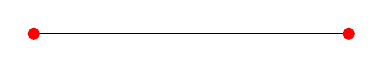
\begin{tikzpicture}
                    % Dibuja el segmento
                    \draw (0,0) -- (4,0);
                    
                    % Dibuja los círculos rojos en los extremos
                    \filldraw[red] (0,0) circle (2pt);
                    \filldraw[red] (4,0) circle (2pt);
                \end{tikzpicture}
            \end{subfigure}
            \begin{subfigure}[c]{0.42\linewidth}
                \centering
                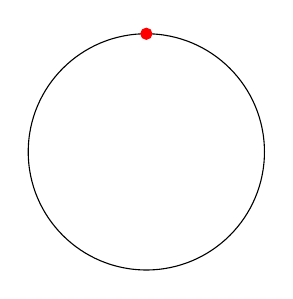
\begin{tikzpicture}
                    % Dibuja la circunferencia
                    \draw (0,0) circle (1.5);
                    
                    % Dibuja el polo norte en rojo
                    \filldraw[red] (0,1.5) circle (2pt);
                \end{tikzpicture}
            \end{subfigure}
            \caption{\centering Identificamos los extremos del segmento con el mismo punto de la circunferencia, ``enrrollando'' entonces el segmento.}
        \end{figure}
        
        
        Sea entonces la relación de equivalencia la siguiente:
        \begin{equation*}
            x\cc{R}y \Longleftrightarrow \left\{\begin{array}{c}
                x=y \\ \lor \\
                \{x,y\} = \{0,1\}
            \end{array}\right.
        \end{equation*}

        

        Consideramos la siguiente aplicación:
        \Func{f}{[0,1]}{\bb{S}^1}{x}{(\cos 2\pi x, \sen 2\pi x)}

        Veamos en primer lugar que $\cc{R}=\cc{R}_f$. Dados $x,y\in [0,1]$, tenemos que:
        \begin{equation*}
            \begin{split}
                x\cc{R}_fy \Longleftrightarrow &f(x)=f(y) \Longleftrightarrow
                \left(\cos 2\pi x, \sen 2\pi x\right) = \left(\cos 2\pi y, \sen 2\pi y\right) \Longleftrightarrow \\
                &\Longleftrightarrow 2\pi x = 2\pi y + 2\pi k,~~k\in \bb{Z}
                \Longleftrightarrow \\
                &\Longleftrightarrow  x = y + k,~~k\in \bb{Z} 
                \Longleftrightarrow  |x - y| = k,~~k\in \bb{N}\cup \{0\}
                \stackrel{(\ast)}\Longleftrightarrow x\cc{R}y
            \end{split}
        \end{equation*}
        donde en $(\ast)$ hemos aplicado que $x,y\in [0,1]$.

        Veamos ahora que $f$ es una identificación. Claramente, $f$ es sobreyectiva. Además, $f$ es continua; y por el lema anterior sabemos que $f$ es cerrada. Por tanto, $f$ es una identificación.

        \item Consideramos la Cinta de Moebius o Möbius, representada en la figura \ref{fig:CintaMoebius}.
        \begin{figure}[H]
            \centering
            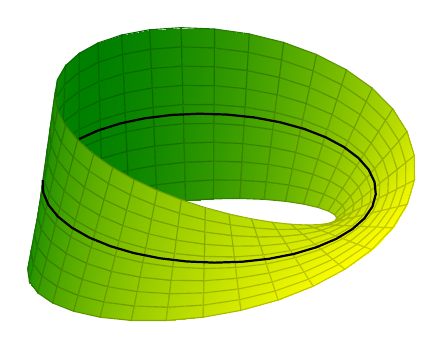
\begin{tikzpicture}
                \begin{axis}[
                    hide axis,
                    view={40}{40}
                ]
                \addplot3 [
                    surf, shader=faceted interp,
                    point meta=x,
                    colormap/greenyellow,
                    samples=35,
                    samples y=10,
                    z buffer=sort,
                    domain=0:360,
                    y domain=-0.5:0.5
                ] (
                    {(1+0.5*y*cos(x/2)))*cos(x)},
                    {(1+0.5*y*cos(x/2)))*sin(x)},
                    {0.5*y*sin(x/2)});
                
                \addplot3 [
                    samples=35,
                    domain=-145:180, % The domain needs to be adjusted manually, depending on the camera angle, unfortunately
                    thick,
                    samples y=1
                ] (
                    {cos(x)},
                    {sin(x)},
                    {0});
                \end{axis}
            \end{tikzpicture}
            \caption{Cinta de Moebius.}
            \label{fig:CintaMoebius}
        \end{figure}

        La definimos como un espacio cociente. Sea el conjunto $[0,1]\times [0,1]$, y definimos la relación de equivalencia $\cc{R}$, vista gráficamente en la figura \ref{fig:CintaMoebius_R}:
        \begin{equation*}
            (x_1,x_2)\cc{R}(y_1,y_2) \Longleftrightarrow \left\{\begin{array}{c}
                (x_1,x_2)=(y_1,y_2) \\ \lor \\
                \{x_1,y_1\} =\{0,1\} \land x_2+y_2=1
            \end{array}\right.
        \end{equation*}
        \begin{figure}[H]
            \centering
            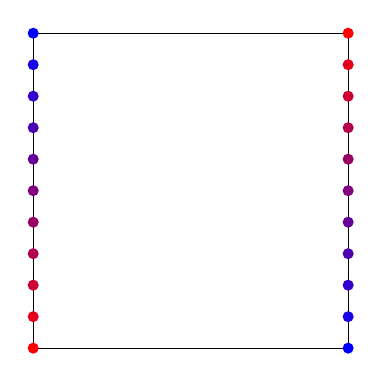
\begin{tikzpicture}
                % Dibuja el rectángulo
                \draw (0,0) rectangle (4,4);
                
                % Dibuja 10 puntos intermedios en color naranja
                \foreach \i in {0,1,...,10} {
                    \pgfmathsetmacro\intensity{int(100 - \i*10)} % Ajusta la intensidad de color
                    \fill[red!\intensity!blue] (0,2*\i/5) circle (2pt);
                    \fill[red!\intensity!blue] (4,4-2*\i/5) circle (2pt);
                }
            \end{tikzpicture}
            \caption{\centering Identificamos cada punto del lado izquierdo con el opuesto del lado derecho.}
            \label{fig:CintaMoebius_R}
        \end{figure}

        La cinta de Moebius se define entonces como el siguiente espacio cociente:
        \begin{equation*}
            \left([0,1]\times [0,1]/\cc{R}, {\T_u}_{[0,1]\times [0,1]}/\cc{R}\right)
        \end{equation*}

        \item Consideramos el toro, representado el la figura \ref{fig:Toro}.
        \begin{figure}[H]
            \centering
            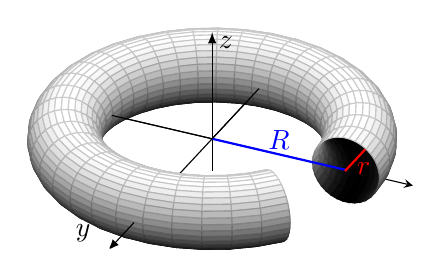
\begin{tikzpicture}
              \begin{axis}[
                  axis equal image,
                  axis lines=middle,
                  xmax=18,zmax=5,
                  ticks=none,
                  clip bounding box=upper bound,
                  colormap/blackwhite
                ]
            
                \addplot3[domain=0:360,y domain=0:320, samples=35,surf,z buffer=sort]
                ({(12 + 3 * cos(x)) * cos(y)} ,
                {(12 + 3 * cos(x)) * sin(y)},
                {3 * sin(x)});
                % use axis coordinate system to draw the radii
                \draw [thick,blue] (axis cs: 0,0,0) -- (axis cs: 12,0,0) node [midway,above=-2] {$R$};
                \draw [thick,red] (axis cs: 12,-0.2,0) -- (axis cs: 12,3.7,0) node [midway,below right=-3] {$r$};
            
                % use axis coordinate system to draw fake x, y and z axes
                \draw [-latex] (axis cs: 0,0,0) -- node [pos=0.9, xshift=0.5em]{$z$}(axis cs: 0,0,10);
                \draw [-latex] (axis cs: 0,-15,0) --
                node [pos=0.9, xshift=-1em, yshift=0.5em]{$y$}(axis cs: 0,-20,0);
                \draw (axis cs: 0,0,0) -- (axis cs: 0,9,0);
                \draw (axis cs: 0,0,0) -- (axis cs: -9,0,0);
              \end{axis}
            \end{tikzpicture}
            \caption{Toro}
            \label{fig:Toro}
        \end{figure}

        Veamos cuál es su ecuación. Para ello, realizamos un corte al toro por el plano $y=0$, y tenemos lo siguiente:
        \begin{figure}[H]
            \centering
            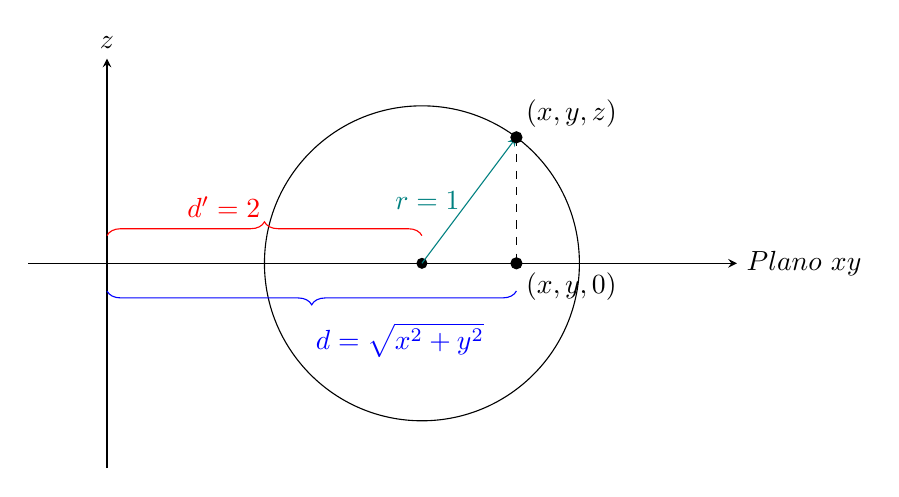
\begin{tikzpicture}[scale=2]
                % Eje horizontal
                \draw[-stealth] (-0.5,0) -- (4,0) node[right] {$Plano~xy$};
                % Eje vertical (A)
                \draw[-stealth] (0,-1.3) -- (0,1.3) node[above] {$z$};

                \def\r{1}
                \def\R{2}

                \coordinate (P) at (2.6,0.8);
                \coordinate (Q) at (2.6,0);
                \coordinate (O) at (\R,0);
                % Dibuja la circunferencia
                \draw (O) circle [radius=\r];
                % Marca el centro de la circunferencia
                \fill (O) circle [radius=1pt];% node[below] {$(2,0)$};
                
                % Etiqueta el radio
                \draw[-stealth, teal] (O) -- (P) node[midway, left] {$r=1$};
                % Punto en la circunferencia P(2.6,0.8)
                \filldraw (P) circle [radius=1pt] node[above right] {$(x,y,z)$};
                
                % Proyeccion del P
                \filldraw (Q) circle [radius=1pt] node[below right] {$(x,y,0)$};

                \draw[dashed] (P) -- (Q);

                % Cota con recta hacia abajo
                \draw[decorate,decoration={brace,amplitude=5pt,mirror},xshift=0pt,yshift=-5pt, blue]
                (0,0) -- (2.6,0) node[midway,below right,yshift=-8pt, xshift=-2pt] {$d=\sqrt{x^2+y^2}$};

                \draw[decorate,decoration={brace,amplitude=5pt},xshift=0pt,yshift=5pt, red]
                (0,0) -- (2,0) node[midway,above left,yshift=3pt, xshift=2pt] {$d'=2$};
            \end{tikzpicture}
        \end{figure}
        Tomamos $(x,y,z)\in \bb{R}^3$. Este estará en el toro de rotación de la circunferencia de radio $r=1$ a una distancia $R=2$ del eje de rotación $z$ si y solo si cumple el Teorema de Pitágoras del triángulo inscrito. Es decir:
        \begin{equation*}
            \left(\sqrt{x^2+y^2}-2\right)^2 + z^2= 1
        \end{equation*}

        \begin{figure}[H]
            \centering
            \begin{subfigure}[c]{0.25\linewidth}
                \centering
                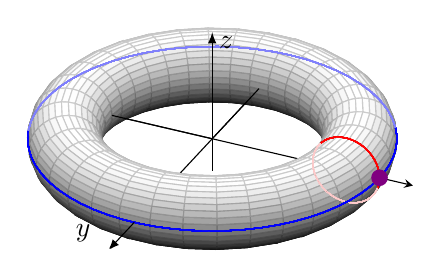
\begin{tikzpicture}
                    \begin{axis}[
                        axis equal image,
                        axis lines=middle,
                        xmax=18, zmax=5,
                        ticks=none,
                        clip bounding box=upper bound,
                        colormap/blackwhite
                    ]
                    
                    \addplot3[domain=0:360, y domain=0:360, samples=35, surf, z buffer=sort]
                    ({(12 + 3 * cos(x)) * cos(y)} ,
                    {(12 + 3 * cos(x)) * sin(y)},
                    {3 * sin(x)});
                
                
                    % Línea roja
                    \addplot3[domain=-20:140, samples=20, surf, z buffer=sort, faceted color=red, opacity=1]
                     ({12+3*cos(x)} ,
                    {0},
                    {3*sin(x)});
                    \addplot3[domain=140:340, samples=20, surf, z buffer=sort, faceted color=red!20, opacity=1]
                     ({12+3*cos(x)} ,
                    {0},
                    {3*sin(x)});
                
                    % Línea azul
                    \addplot3[domain=200:360, samples=30, surf, z buffer=sort, faceted color=blue, opacity=1]
                     ({15*cos(x)} ,
                    {15*sin(x)},
                    {0});
                    \addplot3[domain=0:32, samples=30, surf, z buffer=sort, faceted color=blue, opacity=1]
                     ({15*cos(x)} ,
                    {15*sin(x)},
                    {0});
                    \addplot3[domain=32:200, samples=30, surf, z buffer=sort, faceted color=blue!50, opacity=1]
                     ({15*cos(x)} ,
                    {15*sin(x)},
                    {0});
                    
                    % use axis coordinate system to draw fake x, y and z axes
                    \draw [-latex] (axis cs: 0,0,0) -- node [pos=0.9, xshift=0.5em]{$z$}(axis cs: 0,0,10);
                    \draw [-latex] (axis cs: 0,-15,0) --
                    node [pos=0.9, xshift=-1em, yshift=0.5em]{$y$}(axis cs: 0,-20,0);
                    \draw (axis cs: 0,0,0) -- (axis cs: 0,9,0);
                    \draw (axis cs: 0,0,0) -- (axis cs: -9,0,0);

                    \fill[violet] (axis cs: 15,0,0) circle (3pt);
                    \end{axis}
                \end{tikzpicture}
                \caption{\centering Paso 1. Toro.}
            \end{subfigure}\hspace{2cm}
            \begin{subfigure}[c]{0.25\linewidth}
                \centering
                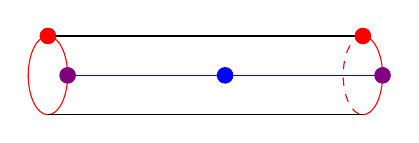
\begin{tikzpicture}
                    % Dibujo del cilindro tumbado
                    \draw[red] (0,0) ellipse (0.25 and 0.5); % Base elíptica
                    \draw[red] (4,-0.5) arc (-90:90:0.25 and 0.5); % Borde superior  
                    \draw[dashed, red] (4, 0.5) arc (90:270:0.25 and 0.5); % Borde superior
                    \draw (0,0.5) -- (4,0.5); % Línea izquierda
                    \draw (0,-0.5) -- (4,-0.5); % Línea izquierda

                    \draw[blue] (0.25,0) -- (4.25,0);

                    \fill[violet] (0.25,0) circle (3pt);
                    \fill[violet] (4.25,0) circle (3pt);

                    \fill[red] (0,0.5) circle (3pt);
                    \fill[red] (4, 0.5) circle (3pt);
                    
                    \fill[blue] (2.25,0) circle (3pt);
                \end{tikzpicture}
                \caption{\centering Paso 2. Cortamos por la circunferencia roja y obtenemos un cilindro.}
            \end{subfigure}\hfill
            \begin{subfigure}[c]{0.25\linewidth}
                \centering
                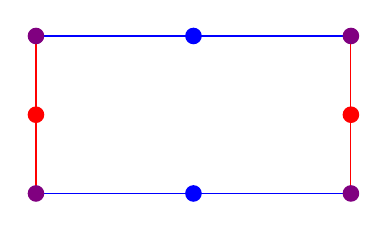
\begin{tikzpicture}
                    \draw[blue] (0,0) -- (4,0);
                    \draw[red] (4,0) -- (4,2);
                    \draw[blue] (4,2) -- (0,2);
                    \draw[red] (0,2) -- (0,0);

                    \fill[violet] (0,0) circle (3pt);
                    \fill[violet] (4,0) circle (3pt);
                    \fill[violet] (4,2) circle (3pt);
                    \fill[violet] (0,2) circle (3pt);

                    \fill[red] (0,1) circle (3pt);
                    \fill[red] (4,1) circle (3pt);

                    \fill[blue] (2,0) circle (3pt);
                    \fill[blue] (2,2) circle (3pt);
                \end{tikzpicture}
                \caption{\centering Paso 3. Cortamos por la recta azul y obtenemos un rectángulo.}
            \end{subfigure}
            \caption{\centering Identificaciones usadas en $\cc{R}$.}
            \label{fig:Toro_R}
        \end{figure}

        Vamos a ver que el toro es homeomorfo a un cociente. Consideramos el cuadrado $[0,1]\times [0,1]\subset \bb{R}^2$ y la siguiente relación de equivalencia, descrita gráficamente en la Figura \ref{fig:Toro_R}:
        \begin{equation*}
            (x_1,x_2)\cc{R}(y_1,y_2) \Longleftrightarrow \left\{\begin{array}{c}
                (x_1,x_2)=(y_1,y_2) \\ \lor \\
                \{x_1,y_1\} =\{0,1\} \land x_2=y_2\\ \lor \\
                \{x_2,y_2\} =\{0,1\} \land x_1=x_2
                \\ \lor \\
                \{x_1,y_1\} =\{0,1\} \land \{x_2,y_2\} =\{0,1\}
            \end{array}\right.
        \end{equation*}

        Queremos probar que $\left([0,1]\times [0,1]/\cc{R}, \T_u/\cc{R}\right)$ es homeomorfo al toro de $\bb{R}^3$ de rotación con su topología usual.

        Buscamos entonces una parametrización del toro. Si $(x,y,z)$ están en el toro, entonces $\left(\sqrt{x^2+y^2}-2\right)^2 + z^2= 1$. Por tanto,
        \begin{equation*}
            \left\{\begin{array}{r}
                \sqrt{x^2+y^2}-2 = \cos\theta \\
                z = \sen\theta
            \end{array}\right.
        \end{equation*}

        Análogamente, como $\sqrt{x^2+y^2}-2 = \cos\theta$, entonces $x^2+y^2 = (2+\cos\theta)^2$. Por tanto,
        \begin{equation*}
            \left\{\begin{array}{l}
                x = (2+\cos\theta)\cos\varphi\\
                y = (2+\cos\theta)\sen\varphi\\
            \end{array}\right.
        \end{equation*}

        Es decir, cada punto del toro se puede parametrizar como:
        \begin{equation*}
            \left\{\begin{array}{l}
                x = (2+\cos\theta)\cos\varphi\\
                y = (2+\cos\theta)\sen\varphi\\
                z = \sen\theta
            \end{array}\right. \hspace{1cm} \theta,\varphi\in [0,2\pi[
        \end{equation*}

        Por tanto, siendo $Toro=\left\{(x,y,z)\in \bb{R}^3\mid \left(\sqrt{x^2+y^2}-2\right)^2 + z^2=1\right\}$; definimos:
        \Func{f}{\left([0,1]\times [0,1], \T_u\right)}{(Toro, \T_u)}{(x,y)}{\left((2+\cos(2\pi x))\cos(2\pi y), (2+\cos(2\pi x))\sen(2\pi y), \sen(2\pi x)\right)}

        Veamos en primer lugar que $\cc{R}=\cc{R}_f$. Dados $(x_1,y_1),(x_2,y_2)\in [0,1]\times [0,1]$, tenemos que:
        \begin{equation*}
            \begin{split}
                (x_1,y_1)&\cc{R}_f(x_2,y_2) \Longleftrightarrow f((x_1,y_1))=f((x_2,y_2)) \Longleftrightarrow \\& \Longleftrightarrow
                \left\{
                \begin{array}{rcl}
                    (2+\cos(2\pi x_1))\cos(2\pi y_1) & = & (2+\cos(2\pi x_2))\cos(2\pi y_2)  \\
                    (2+\cos(2\pi x_1))\sen(2\pi y_1) & = & (2+\cos(2\pi x_2))\sen(2\pi y_2) \\
                    \sen(2\pi x_1) & = & \sen(2\pi x_2)
                \end{array}
                \right\}
                \stackrel{(\ast)}{\Longleftrightarrow} \\& \Longleftrightarrow
                \left\{
                \begin{array}{rcl}
                     \sen(2\pi x_1) & = & \sen(2\pi x_2) \\
                     \cos(2\pi x_1) & = & \cos(2\pi x_2) \\
                     \cos(2\pi y_1) & = & \cos(2\pi y_2)\\
                     \sen(2\pi y_1) & = & \sen(2\pi y_2)
                \end{array}
                \right\}
                \Longleftrightarrow
                \left\{
                \begin{array}{c}
                     2\pi x_1 = 2\pi x_2 +2k_1\pi \\
                     \land\\
                     2\pi y_1 = 2\pi y_2 +2k_1\pi
                \end{array}
                \right. k_1,k_2\in \bb{Z} \Longleftrightarrow \\
                &\Longleftrightarrow
                \left\{
                \begin{array}{c}
                     x_1-x_2\in \bb{Z}\\
                     \land\\
                     y_1-y_2\in \bb{Z}
                \end{array}
                \right\}
                \Longleftrightarrow
                (x_1,y_1)\cc{R}(x_2,y_2)
            \end{split}
        \end{equation*}
        donde en $(\ast)$ he elevado la primera y segunda ecuación al cuadrado, y luego las he sumado obteniendo:
        \begin{gather*}
            \left\{
            \begin{array}{rcl}
                (2+\cos(2\pi x_1))^2\cos^2(2\pi y_1) & = & (2+\cos(2\pi x_2))^2\cos^2(2\pi y_2)  \\
                (2+\cos(2\pi x_1))^2\sen^2(2\pi y_1) & = & (2+\cos(2\pi x_2))^2\sen^2(2\pi y_2)
            \end{array}
            \right\} \\
            \hspace{-1.42cm}
            \begin{array}{rcl}
                2(2+\cos(2\pi x_1))^2[\cos^2(2\pi y_1)+\sen^2(2\pi y_1] & = & 2(2+\cos(2\pi x_2))^2[\cos^2(2\pi y_2)+\sen^2(2\pi y_2)]
            \end{array}
             \\
            \begin{array}{rcl}
                (2+\cos(2\pi x_1))^2 & = & (2+\cos(2\pi x_2))^2
            \end{array}
            \\
            \begin{array}{rcl}
                \cos(2\pi x_1) & = & \cos(2\pi x_2)
            \end{array}
        \end{gather*}

        Veamos ahora que $f$ es una identificación. Claramente, $f$ es sobreyectiva. Además, $f$ es continua (porque cada coordenada lo es); y por el lema anterior sabemos que $f$ es cerrada. Por tanto, $f$ es una identificación.

        Por tanto, $f$ induce un homeomorfismo $\wt{f}:\left([0,1]\times [0,1]/\cc{R}, \T_u/\cc{R}\right)\to (Toro, \T_u)$.

        \item Observemos que el toro también es homeomorfo a $\left(\bb{S}^1\times \bb{S}^1/\cc{R}, {\T_u^4}_{\bb{S}^1\times \bb{S}^1}/\cc{R}\right)$.


        Por el primer ejemplo visto en este apartado, $\left([0,1]/\cc{R},{\T_u}_{[0,1]}/\cc{R}\right)\cong (\bb{S}^1,{\T_u}_{\bb{S}^1})$. Entonces:
        \begin{equation*}
            \left([0,1]\times [0,1]/\cc{R},{\T_u}/\cc{R}\right)\cong \left(\bb{S}^1\times \bb{S}^1/\cc{R}, {\T_u^4}_{\bb{S}^1\times \bb{S}^1}/\cc{R}\right)
        \end{equation*}


        Como el Toro es homeomorfo a $\left([0,1]\times [0,1]/\cc{R}, \T_u/\cc{R}\right)$, entonces por transitividad es homeomorfo a $\left(\bb{S}^1\times \bb{S}^1/\cc{R}, {\T_u^4}_{\bb{S}^1\times \bb{S}^1}/\cc{R}\right)$.

        Análogamente, se podría demostrar haciendo uso de la siguiente identificación:
        \Func{f}{\left(\bb{S}^1\times \bb{S}^1, {\T_u^4}_{\bb{S}^1\times \bb{S}^1}\right)}{(Toro, \T_u)}{(x_1,x_2,x_3,x_4)}{\left((2+x_1)x_3, (2+x_1)x_4, x_2\right)}
        
        \item \ul{El espacio proyectivo (real)}.

        Tomamos $X=\bb{R}^n\setminus \left\{\vec{0}\right\}$, y consideramos la relación de equivalencia:
        \begin{equation*}
            x\cc{R}y \Longleftrightarrow \exists\lm \in \bb{R}^\ast\mid y =\lm x 
        \end{equation*}

        Al espacio cociente $X/\cc{R}$ se le llama espacio proyectivo real, y lo denominaremos $\bb{R}P^{n-1}$. Notemos que nosotros consideraremos sobre el espacio proyectivo siempre la topología usual.

        También podemos considerar sobre $\bb{S}^n\subset \bb{R}^{n+1}$ la relación de equivalencia:
        \begin{equation*}
            x\ol{\cc{R}}y \Longleftrightarrow x=\pm y
        \end{equation*}

        
        Veamos que $\left(\bb{R}^{n+1}\setminus \left\{\vec{0}\right\}/\cc{R}, \T_u/\cc{R}\right)$ es homeomorfo a $(\bb{S}^n/\ol{\cc{R}}, \T_u/\ol{\cc{R}})$. Sea la siguiente aplicación:
        \Func{F}{\left(\bb{R}^{n+1}\setminus \left\{\vec{0}\right\}, \T_u\right)}{(\bb{S}^n, \T_u)}{x}{\dfrac{x}{\|x\|}}

        Tenemos entonces el siguiente diagrama de composiciones:
        \begin{figure}[H]
            \centering
            \shorthandoff{""}
            \begin{tikzcd}
            \bb{R}^{n+1} \setminus\left\{\vec{0}\right\}\arrow[r, "F"] \arrow[d, "{p}"'] \arrow[rd, "\ol{p}\circ F"] & \bb{S}^n  \arrow[d, "\ol{p}"] \\
            \bb{R}^{n+1}\setminus\left\{\vec{0}\right\}/\cc{R} \arrow[r, "\wt{F}"']                            &         \bb{S}^n/\ol{\cc{R}}
            \end{tikzcd}
            \shorthandon{""}
        \end{figure}

        Veamos que $F$ se induce en los cocientes a $\wt{F}:\bb{R}^{n+1}-\left\{\vec{0}\right\}/\cc{R}\to \bb{S}^n/\ol{\cc{R}}$. Para ello, vemos en primer lugar que $\wt{F}$ está bien definida. Es decir, si $x\cc{R}y$, entonces $(\ol{p}\circ F)(x) = (\ol{p}\circ F)(y)$.
        \begin{multline*}
            x\cc{R}y \Longrightarrow x=\lambda y,~\lm \neq 0 \Longrightarrow F(x)=F(\lm y) \Longrightarrow \frac{x}{\|x\|} = \frac{\lm y}{\|\lm y\|} = \pm \frac{y}{\|y\|} \Longrightarrow \\ \Longrightarrow F(x) = \pm F(y) \Longrightarrow F(x)\ol{\cc{R}}F(y) \Longrightarrow (\ol{p}\circ F)(x) = (\ol{p}\circ F)(y)
        \end{multline*}

        Por tanto, $\wt{F}$ está bien definida. Veamos que $\wt{F}$ es un homeomorfismo. Tenemos que $\wt{F}$ es continua si y solo si lo es $\wt{F}\circ p$ es continua, ya que $p$ es una identificación. No obstante, $\wt{F}\circ p = \ol{p}\circ F$, que es composición de dos continuas, por lo que $\wt{F}$ es continua.


        Busquemos ahora su inversa. Sea la siguiente aplicación:
        \Func{i=G}{\bb{S}^n}{\bb{R}^{n+1}\setminus \left\{\vec{0}\right\}}{x}{x}

        Veamos que $G$ se induce a $\wt{G}:\bb{S}^n/\ol{\cc{R}}\to \bb{R}^{n+1}\setminus \left\{\vec{0}\right\}/\cc{R}$.
        \begin{figure}[H]
            \centering
            \shorthandoff{""}
            \begin{tikzcd}
            \bb{S}^n \arrow[r, "G"] \arrow[d, "\ol{p}"'] \arrow[rd, "p\circ G"] & \bb{R}^{n+1}\setminus\left\{\vec{0}\right\} \arrow[d, "p"] \\
            \bb{S}^n/\ol{\cc{R}} \arrow[r, "\wt{G}"]                            & \bb{R}^{n+1}\setminus\left\{\vec{0}\right\}/\cc{R}        
            \end{tikzcd}
            \shorthandon{""}
        \end{figure}
        Tenemos que ver que $\wt{G}$ está bien definida; es decir, si $x,y\in \bb{S}^n\mid x\ol{\cc{R}}y$, entonces $p(G(x))=p(G(y))$.
        \begin{equation*}
            x\ol{\cc{R}}y \Longrightarrow x=\pm y\Longrightarrow G(x) = G(\pm y)\Longrightarrow x=\pm y \Longrightarrow x\cc{R}y \Longrightarrow p(G(x)) = p(G(y))
        \end{equation*}

        Además, Tenemos que $\wt{G}$ es continua si y solo si lo es $\wt{G}\circ \ol{p}$ es continua, ya que $\ol{p}$ es una identificación. No obstante, $\wt{G}\circ \ol{p} = p\circ G$, que es composición de dos continuas, por lo que $\wt{G}$ es continua.

        Falta probar que $\wt{F}=\wt{G}^{-1}$. Dado $x\in \bb{R}^{n+1}\setminus\left\{\vec{0}\right\}$, tenemos que:
        \begin{equation*}
            \wt{G}(\wt{F}(p(x))) = \wt{G}(\ol{p}(F(x))) = \wt{G}\left(\ol{p}\left(\frac{x}{\|x\|}\right)\right) = p\left(G\left(\frac{x}{\|x\|}\right)\right) = p\left(\frac{x}{\|x\|}\right) = p(x)
        \end{equation*}
        Por lo que $\wt{G}\circ \wt{f}=Id$. Dado $x\in \bb{S}^n$, por lo que $\|x\|=1$:
        \begin{equation*}
            \wt{F}(\wt{G}(\ol{p}(x))) = \wt{F}(p(G(x))) = \wt{F}(p(x)) = \ol{p}(F(x)) = \ol{p}\left(\frac{x}{\|x\|}\right)
            = \ol{p}\left(x\right)
        \end{equation*}
        Por lo que $\wt{F}\circ \wt{G}=Id$, y por tanto $\wt{G}=\wt{F}^{-1}$

        Entonces, tenemos que $\wt{f}$ es un homeomorfismo.
    \end{enumerate}
    
    Introducimos ahora el concepto de cocientes por un subconjunto:
    \begin{definicion}[Cocientes por un subconjunto]
        Dado un espacio topológico $(X,\T)$ y $A\subset X$ subconjuntos cualquiera, se considera la relación de equivalencia:
        \begin{equation*}
            x\cc{R}y \Longleftrightarrow \left\{
            \begin{array}{c}
                x=y \\ \lor \\ x,y\in A
            \end{array}
            \right.
        \end{equation*}

        Se define el espacio cociente por el subconjunto $A$ como el espacio cociente $(X/\cc{R}, \T/\cc{R})$ para la relación de equivalencia $\cc{R}$ anterior.
        Se denota normalmente como:
        \begin{equation*}
            (X/A,\T/A)
        \end{equation*}
    \end{definicion}
    \begin{ejemplo}
        Consideremos $(X,\T)=([-1,1],\T_u)$, y como subconjunto $A=\{-1,0,1\}$. Veamos que $([-1,1]/A,\T_u/A)$ es homeomorfo a dos circunferencias tangentes en un punto:
        \begin{equation*}
            C = \left\{(x,y)\in \bb{R}^2\left|
                \begin{array}{c}
                    (x-1)^2 + y^2=1 \\ \lor \\
                    (x+1)^2 + y^2 = 1
                \end{array}
            \right.\right\}
        \end{equation*}
        \begin{figure}[H]
            \centering
            \begin{tikzpicture}
                % Ejes cartesianos
                \draw[-stealth] (-3,0) -- (3,0) node[right] {$x$};
                \draw[-stealth] (0,-2) -- (0,2) node[above] {$y$};
                
                % Circunferencias
                \draw (1,0) circle (1);
                \draw (-1,0) circle (1);
                
                % Puntos de centro de las circunferencias
                \filldraw (1,0) circle (2pt) node[below] {$1$};
                \filldraw (-1,0) circle (2pt) node[below] {$-1$};
            \end{tikzpicture}
        \end{figure}

        Definimos la aplicación:
        \Func{f}{[-1,1]}{C}{x}{\left\{
        \begin{array}{lcc}
            (1-\cos(2\pi x), \sen(2\pi x)) & \text{si} & 0\leq x\leq 1 \\
            (-1+\cos(2\pi x), \sen(2\pi x)) & \text{si} & -1\leq x\leq 0
        \end{array}
        \right.}

        Por el carácter local de la continuidad, $f$ es continua en $[-1,1]\setminus \{0\}$. Además, mediante límites se comprueba que $f$ es continua en el origen. Además, es biyectiva y; como $[-1,1]$ es cerrado y acotado, es cerrada; por lo que se trata de un homeomorfismo.
        % TERMINAR
    \end{ejemplo}
\end{ejemplo}


\section{Relación de Ejercicios}
Para ver ejercicios relacionados con el Tema 2, consultar la sección \ref{sec:Rel2}.